\chapter{Results and interpretation}
%\minitoc
In this chapter, the results are presented. The analysis was designed and validated before looking at the data in the SRs. Hence, the chapter commences with the results of the validity test~(Sec.~\ref{sec:ResVal}) of the data-driven background prediction in a restricted region spared from the $\wJets$ sideband. It proceeds with the comparison between the background prediction and the observed event yields in the mainband signal regions (Sec.~\ref{sec:Resmain}) and in the aggregated regions (Sec.~\ref{sec:AggrRes}). Following a summary of the statistical procedures, the interpretation of results in the framework of simplified SUSY models is presented. The chapter concludes with a discussion on the comparison of the results with complementary analyses.
\section{Results of the background prediction}
\subsection{Result of the validation in sideband regions}
\label{sec:ResVal}
As mentioned in Sec. \ref{sec:Val}, the background estimation method is validated in regions where the $\njet$ selection is restricted to 4 jets and kinematic requirements in $\LT$ and $\HT$ is aligned with the mainband regions.
Accordingly, the sideband where $\Rcs$ of $\wJets$ events is measured is defined by $\njet$=3 in order to avoid overlap.
This restriction results in a statistical limitation and a slight reduced performance of the method.
The sideband region for measuring $\ttJets$ $\Rcs$ remains unchanged.
%Examples of b-tag multiplicity fit, which are performed for the validation, can be seen in Fig.~\ref{fig:btagMultiplicityFit_val_data}. 
%Fig. \ref{kappaVal} shows the $\kappa$ values for the validation prediction.
Results of this validation are shown in Fig.~\ref{fig:validation_0b}.
The systematic uncertainties shown in this figure are an approximate projection of what is observed in the mainband regions. Figure~\ref{fig:validation_0b} manifests that the data agrees with the SM prediction in the validation regions.
%\begin{figure}[!h]
%\begin{center}
%    \subfigure[$\njet=3$]{ 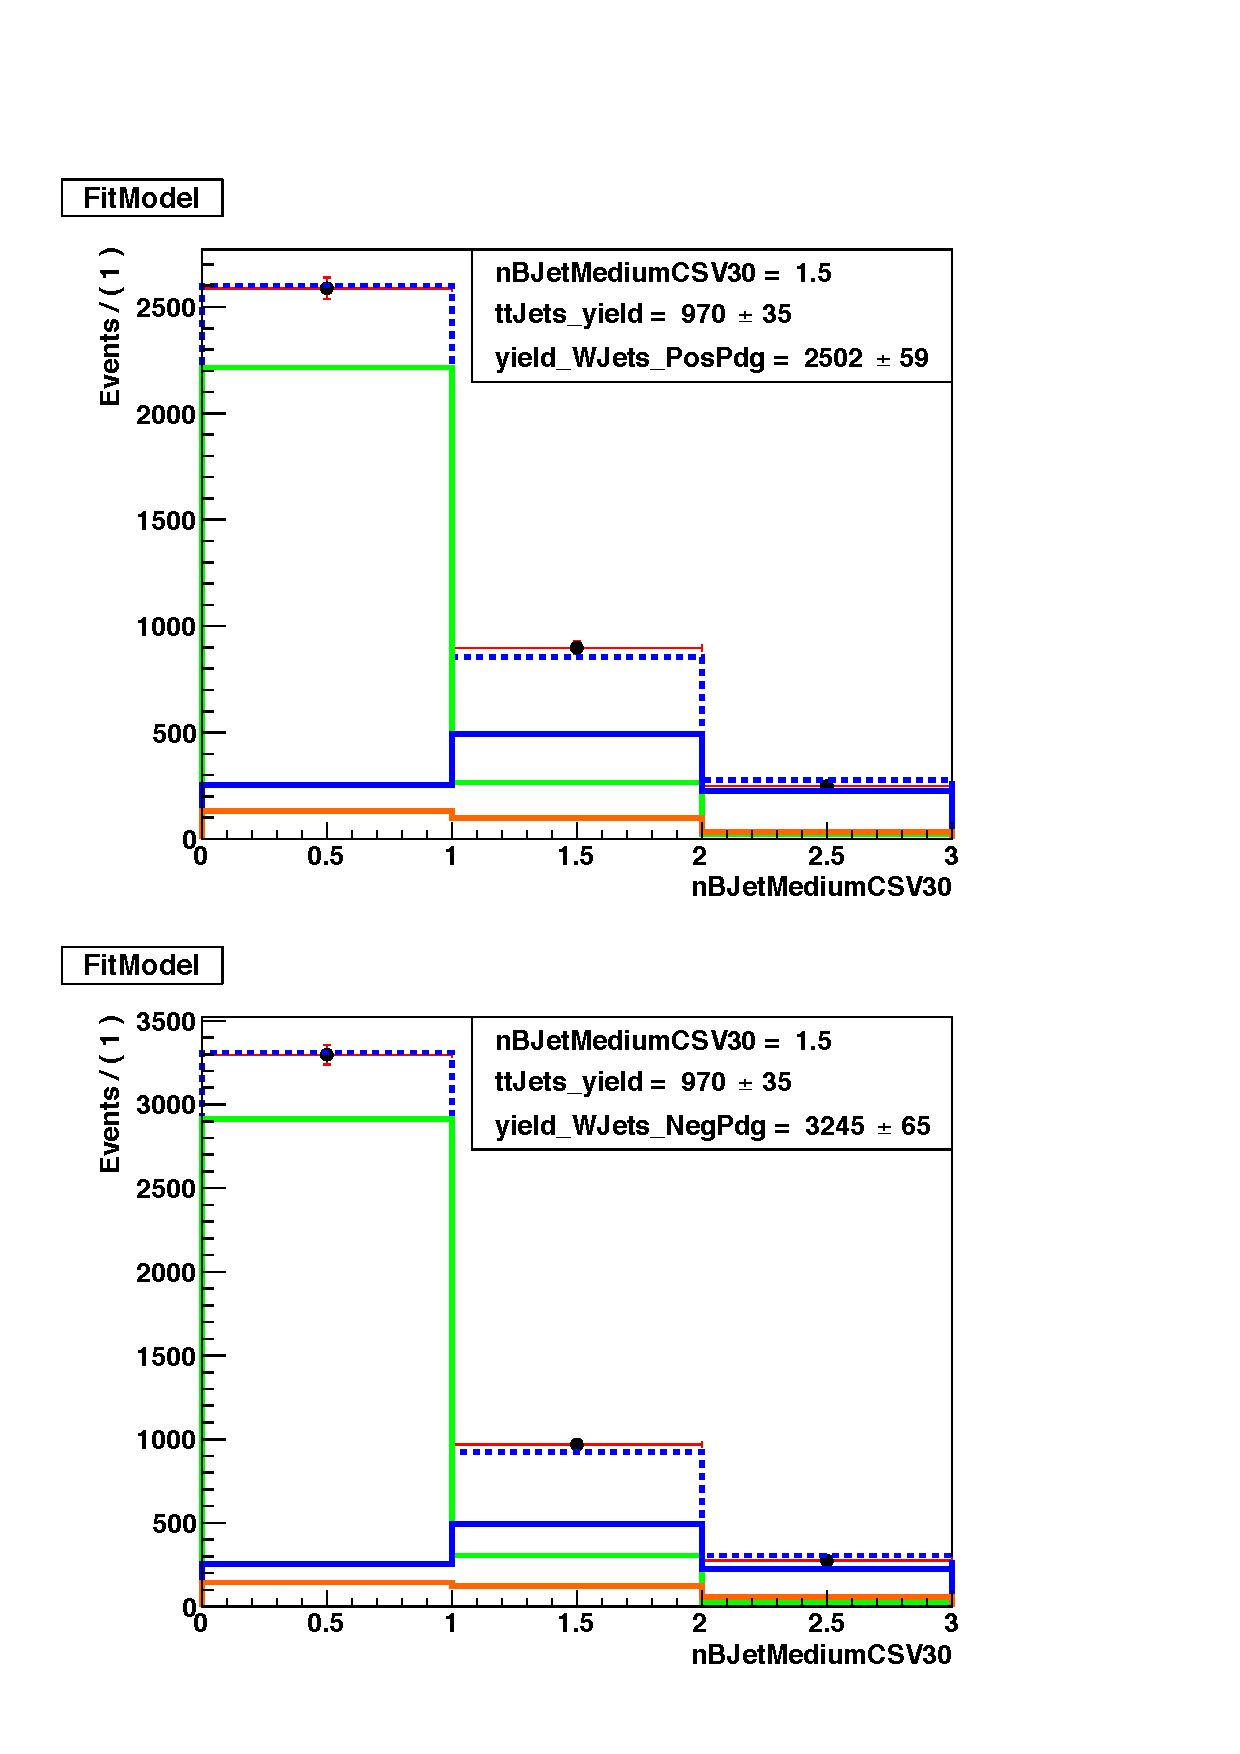
\includegraphics[width=0.4 \textwidth]{Plots/analysis/results/st250-350_ht500-750_njetEq3_nBTagFitRes.pdf}}
    %\subfigure[$\njet=4$]{ 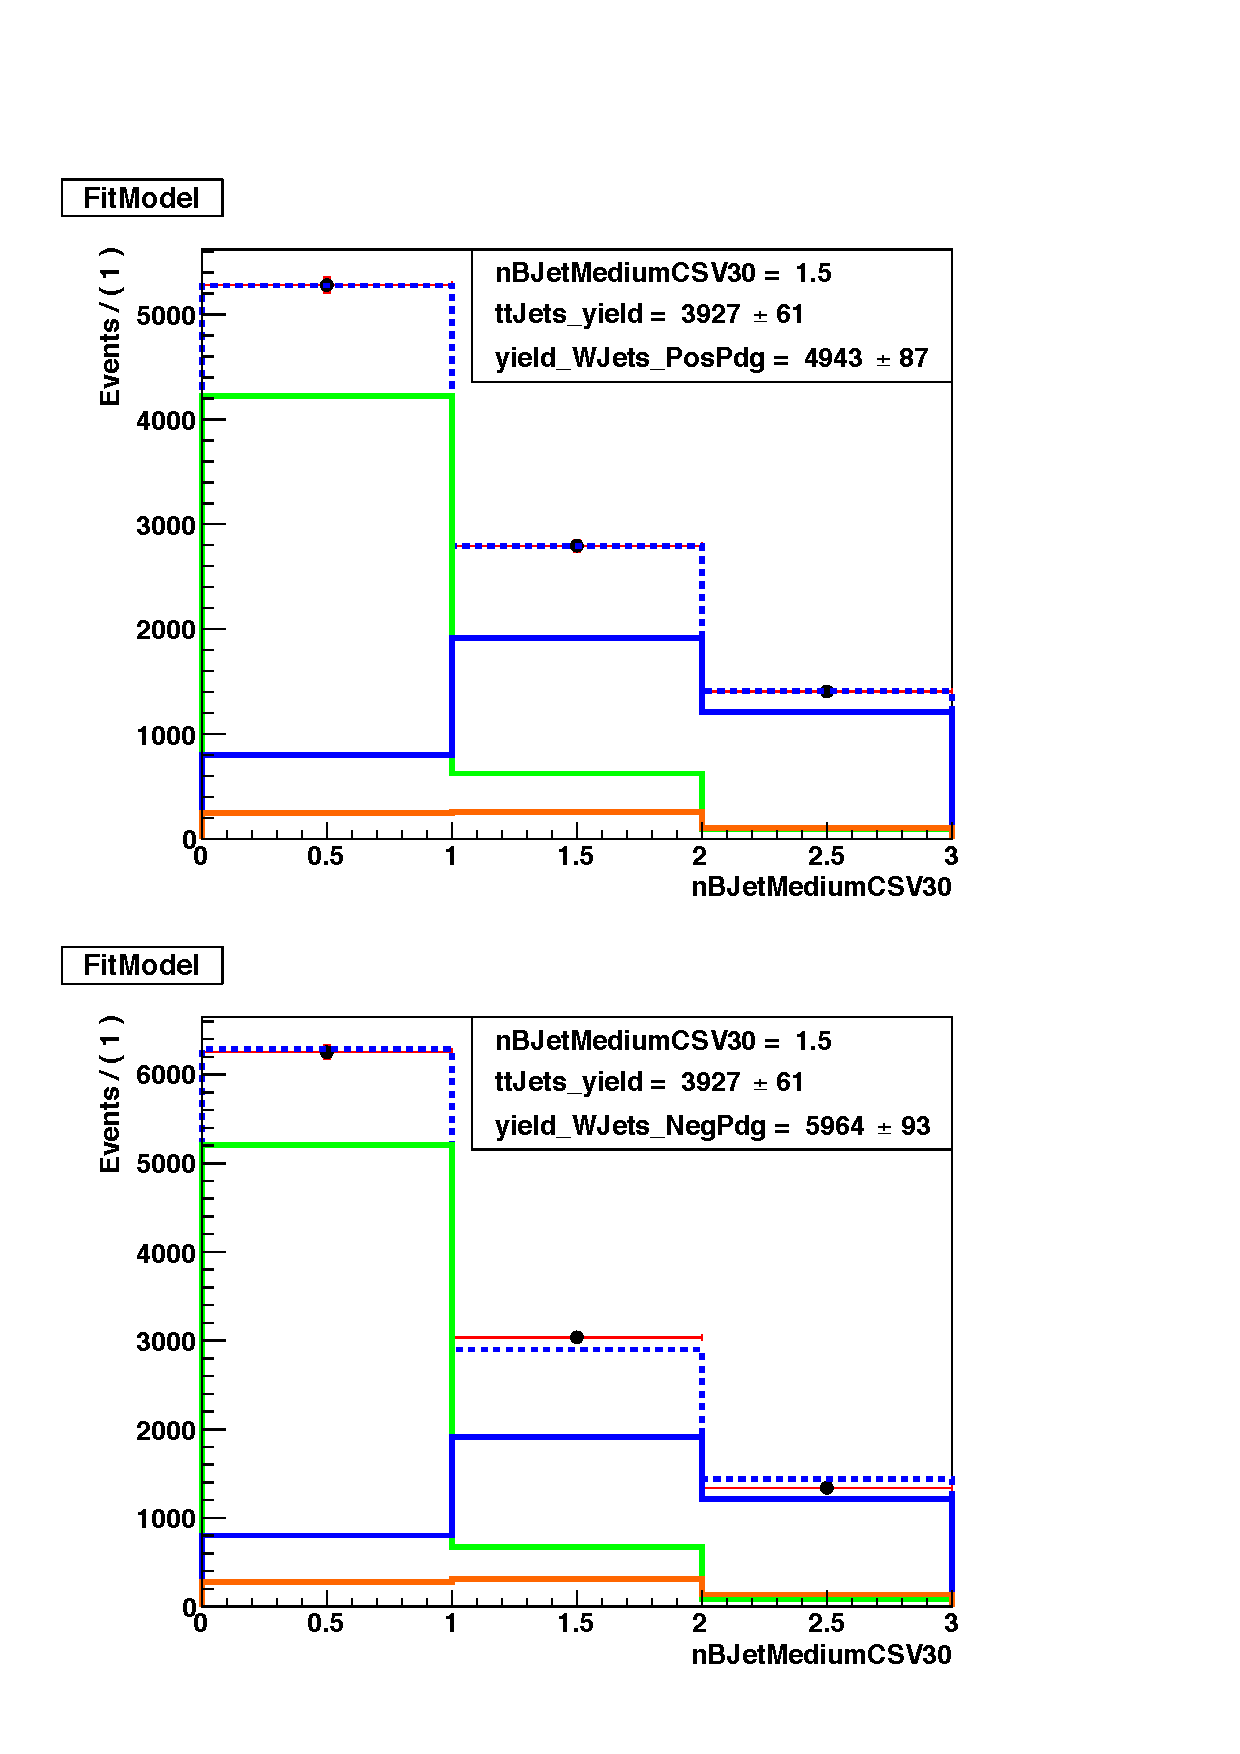
\includegraphics[width=0.4 \textwidth]{Plots/analysis/results/st250-350_ht500-750_njetEq4_nBTagFitRes.pdf}}
    %\caption{Fits to the \nbtag multiplicity for control regions in (a) $\njet = 3$ ($250\leq$\LT$<350\GeV$, \HT$\geq500$GeV, $\DF<1$, muon channel) and (b) $\njet = 4$ ($250\leq$\LT$<350\GeV$, \HT$\geq500\GeV$, $\DF<1$) in data.
%The solid lines represent the templates scaled according to the fit result (blue for $\ttJets$, green for $\wJets$, turquoise for QCD, and red for the remaining backgrounds), the dashed line shows the sum after fit, and the points with error bars represent data.}
%    \label{fig:btagMultiplicityFit_val_data}
%\end{center}
%\end{figure}
\begin{figure}[!h]
\begin{center}
    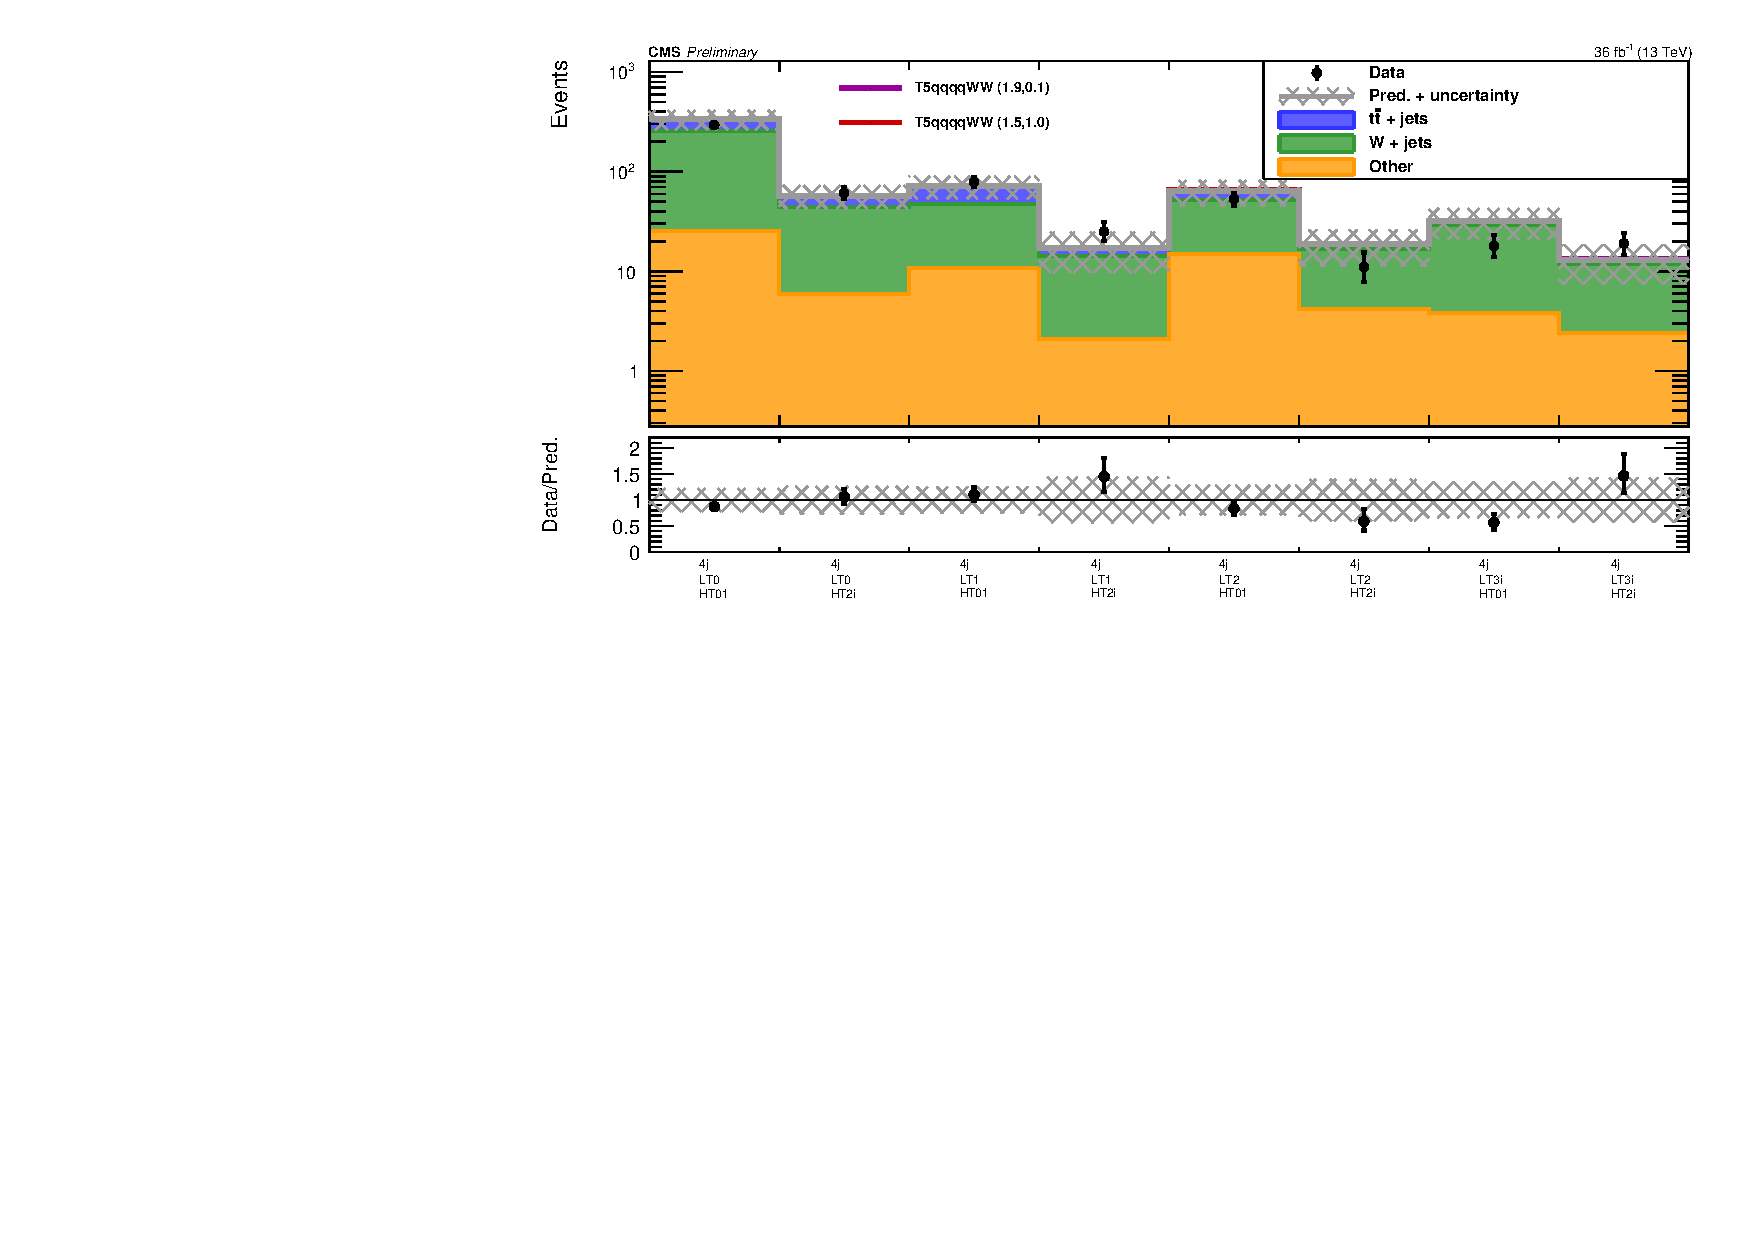
\includegraphics[width=0.9 \textwidth]{Plots/analysis/results/Prediction_Spring16_templates_validation_4j_Moriond2017_lep_data_36p5_blind.pdf}
    \caption[The results of background estimation method validation.]{Validation of the background estimation method, using mainband regions with 4 jets.
    The shaded area reflects a rough estimate of the statistical and systematic uncertainties.
    The colored lines illustrate the expectations for two benchmark points of the T5qqqqWW model, showing the SUSY particle masses m$_{\tilde{g}}$/m$_{\ninozero}$ in TeV.
    The lower band shows the ratio between observed and predicted events.
    }
    \label{fig:validation_0b}
\end{center}
\end{figure}
\subsection{Result of the background prediction in mainband regions}
\label{sec:Resmain}
Figure~\ref{fig:mainRes} shows the observed event yields from data in signal regions for the 28 mainband bins, compared to the data-driven SM background prediction (see Ch.~\ref{chap:Rcs}). 
In figure, the stacked colored histograms represent the prediction corresponding to the individual background contributions grouped into $\ttJets$, $\wJets$ and EWK. \\
No significant deviation from the SM prediction is observed. A summary table of the background prediction and the final observed yields for each 28 bin can be found in Tab.~\ref{tab:main_results}.
The distributions of $\DF$ in data and simulation are shown in Fig.~\ref{fig:DFunblind} for the four $\LT$ intervals after the baseline selection with inclusive requirements on $\njet\geq$ 5 and $\HT\geq$ 500 GeV. Overall, data and the SM simulation is also in good agreement in this inclusive regions. Although, this agreement is not a necessity for the analysis flow, it confirms the reliability of the simulation based $\kappa$ factors.
\begin{table*}[!ht]
\centering
\caption{Summary of the results in the main search regions. The $\DF$ value that is used to define the CR and SR is given as well.}
\label{tab:main_results}
\resizebox{\textwidth}{!}{\begin{tabular}{c|c|c|c|l|rrr|lll|rrr|c}
    \multirow{2}{*}{\njet}     & \LT & \DF& \HT     & Bin & \multicolumn{6}{c|}{Signal T5qqqqWW ($m_{\PSg}$, $m_{\PSGcz}$) $[$TeV$]$} & \multicolumn{3}{c|}{Predicted} & \multirow{2}{*}{Observed} \\%\hline
 & $[$GeV$]$ &[rad]  &$[$GeV$]$ &  name & \multicolumn{3}{c}{(1.5, 1.0)} & \multicolumn{3}{c|}{(1.9, 0.1)} & \multicolumn{3}{c|}{background} &  \\\hline
\hline
$5$
&$[250,350]$ & 1.0
&$[500,750]$
 & G01
  & 1.82&$\pm$&0.29 & \multicolumn{3}{c|}{$<0.01$}& 101.91&$\pm$&47.55
 & 111 \\
\cline{4-15}
& &
&$\geq750$
 & G02
 & 0.21&$\pm$&0.09 & 0.01&$\pm$&0.01 & 76.73&$\pm$&16.19
 & 100 \\
\cline{2-15}
&$[350,450]$ & 1.0
&$[500,750]$
 & G03
& 2.25&$\pm$&0.32 & \multicolumn{3}{c|}{$<0.01$}& 24.43&$\pm$&14.78
 & 25 \\
\cline{4-15}
& &
&$\geq750$
 & G04
 & 0.29&$\pm$&0.11 & 0.04&$\pm$&0.01 & 22.78&$\pm$&8.29
 & 22 \\
\cline{2-15}
&$[450,650]$ & 0.75
&$[500,750]$
 & G05
& 3.02&$\pm$&0.37 & \multicolumn{3}{c|}{$<0.01$}& 14.46&$\pm$&6.5
 & 17 \\
\cline{4-15}
& &
&$[750,1250]$
 & G06
 & 1.4&$\pm$&0.25 & 0.04&$\pm$&0.02 & 12.13&$\pm$&4.68
 & 10 \\
\cline{4-15}
&&
&$\geq1250$
 & G07
 & 0.08&$\pm$&0.06 & 0.25&$\pm$&0.04 & 4.15&$\pm$&1.72
 & 2 \\
\cline{2-15}
&$\geq650$ & 0.5
&$[500,750]$
 & G08
 & 0.74&$\pm$&0.18 & 0.01&$\pm$&0.01 & 2.32&$\pm$&1.49
 & 5 \\
\cline{4-15}
& &
&$[750,1250]$
 & G00
 & 0.49&$\pm$&0.15 & 0.12&$\pm$&0.03 & 5.79&$\pm$&1.96
 & 6 \\
\cline{4-15}
& &
&$\geq1250$
 & G10
 & 0.14&$\pm$&0.07 & 1.15&$\pm$&0.08 & 2.74&$\pm$&1.26
 & 0 \\
\cline{2-15}
\hline
\hline
$[6,7]$
&$[250,350]$ & 1.0
&$[500,1000]$
 & H01
  & 3.02&$\pm$&0.36 & \multicolumn{3}{c|}{$<0.01$}& 89.32&$\pm$&38.21
 & 85 \\
\cline{4-15}
& &
&$\geq1000$
 & H02
 & 0.31&$\pm$&0.1 & 0.09&$\pm$&0.02 & 30.94&$\pm$&5.08
 & 33 \\
\cline{2-15}
&$[350,450]$ & 1.0
&$[500,1000]$
 & H03
 & 4.13&$\pm$&0.41 & 0.01&$\pm$&0.01 & 18.91&$\pm$&10.89
 & 31 \\
\cline{4-15}
& &
&$\geq1000$
 & H04
 & 0.52&$\pm$&0.14 & 0.14&$\pm$&0.03 & 9.51&$\pm$&2.34
 & 8 \\
\cline{2-15}
&$[450,650]$ & 0.75
&$[500,750]$
 & H05
& 3.63&$\pm$&0.39 & \multicolumn{3}{c|}{$<0.01$}& 5.71&$\pm$&3.31
 & 13 \\
\cline{4-15}
& &
&$[750,1250]$
 & H06
 & 3.79&$\pm$&0.39 & 0.03&$\pm$&0.01 & 8.21&$\pm$&3.15
 & 8 \\
\cline{4-15}
&&
&$\geq1250$
 &  H07
 & 0.36&$\pm$&0.12 & 0.47&$\pm$&0.05 & 3.61&$\pm$&1.78
 & 4 \\
\cline{2-15}
&$\geq650$ & 0.5
&$[500,750]$
 & H08
& 0.89&$\pm$&0.19 & \multicolumn{3}{c|}{$<0.01$}& 0.79&$\pm$&0.53
 & 3 \\
\cline{4-15}
& &
&$[750,1250]$
 & H09
 & 1.77&$\pm$&0.26 & 0.15&$\pm$&0.03 & 3.63&$\pm$&1.37
 & 5 \\
\cline{4-15}
&&
&$\geq1250$
 & H10
 & 0.83&$\pm$&0.18 & 2.83&$\pm$&0.12 & 1.83&$\pm$&0.86
 & 1 \\
\cline{2-15}
\hline
\hline
$\geq8$
&$[250,350]$ & 1.0
&$[500,1000]$
 & I01
  & 0.88&$\pm$&0.18 & \multicolumn{3}{c|}{$<0.01$}& 6.96&$\pm$&2.83
 & 16 \\
\cline{4-15}
& &
&$\geq1000$
 & I02
 & 0.26&$\pm$&0.09 & 0.03&$\pm$&0.01 & 6.32&$\pm$&1.17
 & 4 \\
\cline{2-15}
&$[350,450]$ & 1.0
&$[500,1000]$
 & I03
& 0.55&$\pm$&0.14 & \multicolumn{3}{c|}{$<0.01$}& 1.67&$\pm$&0.77
 & 3 \\
\cline{4-15}
& &
&$\geq1000$
 & I04
 & 0.72&$\pm$&0.15 & 0.11&$\pm$&0.02 & 2.65&$\pm$&0.89
 & 4 \\
\cline{2-15}
&$[450,650]$ &0.75
&$[500,1250]$
 & I05
 & 2.07&$\pm$&0.26 & 0.01&$\pm$&0.01 & 0.63&$\pm$&0.32
 & 0 \\
\cline{4-15}
&&
&$\geq1250$
 & I06
 & 0.45&$\pm$&0.12 & 0.3&$\pm$&0.04 & 0.68&$\pm$&0.35
 & 1 \\
\cline{2-15}
&$\geq650$ & 0.5
&$[500,1250]$
 & I06
 & 0.97&$\pm$&0.18 & 0.04&$\pm$&0.01 & 0.27&$\pm$&0.23
 & 1 \\
\cline{4-15}
&&
&$\geq1250$
 & I07
 & 1.12&$\pm$&0.18 & 1.37&$\pm$&0.08 & 0.38&$\pm$&0.24
 & 1 \\
\cline{2-15}\hline
\end{tabular}}
\end{table*}
%Additionally, all the components of the background prediction such as the data yields in the sideband SR and CR, predicted QCD background contamination and various $\kappa$ factors are listed.\\
\begin{figure}[!htb]
\begin{center}
    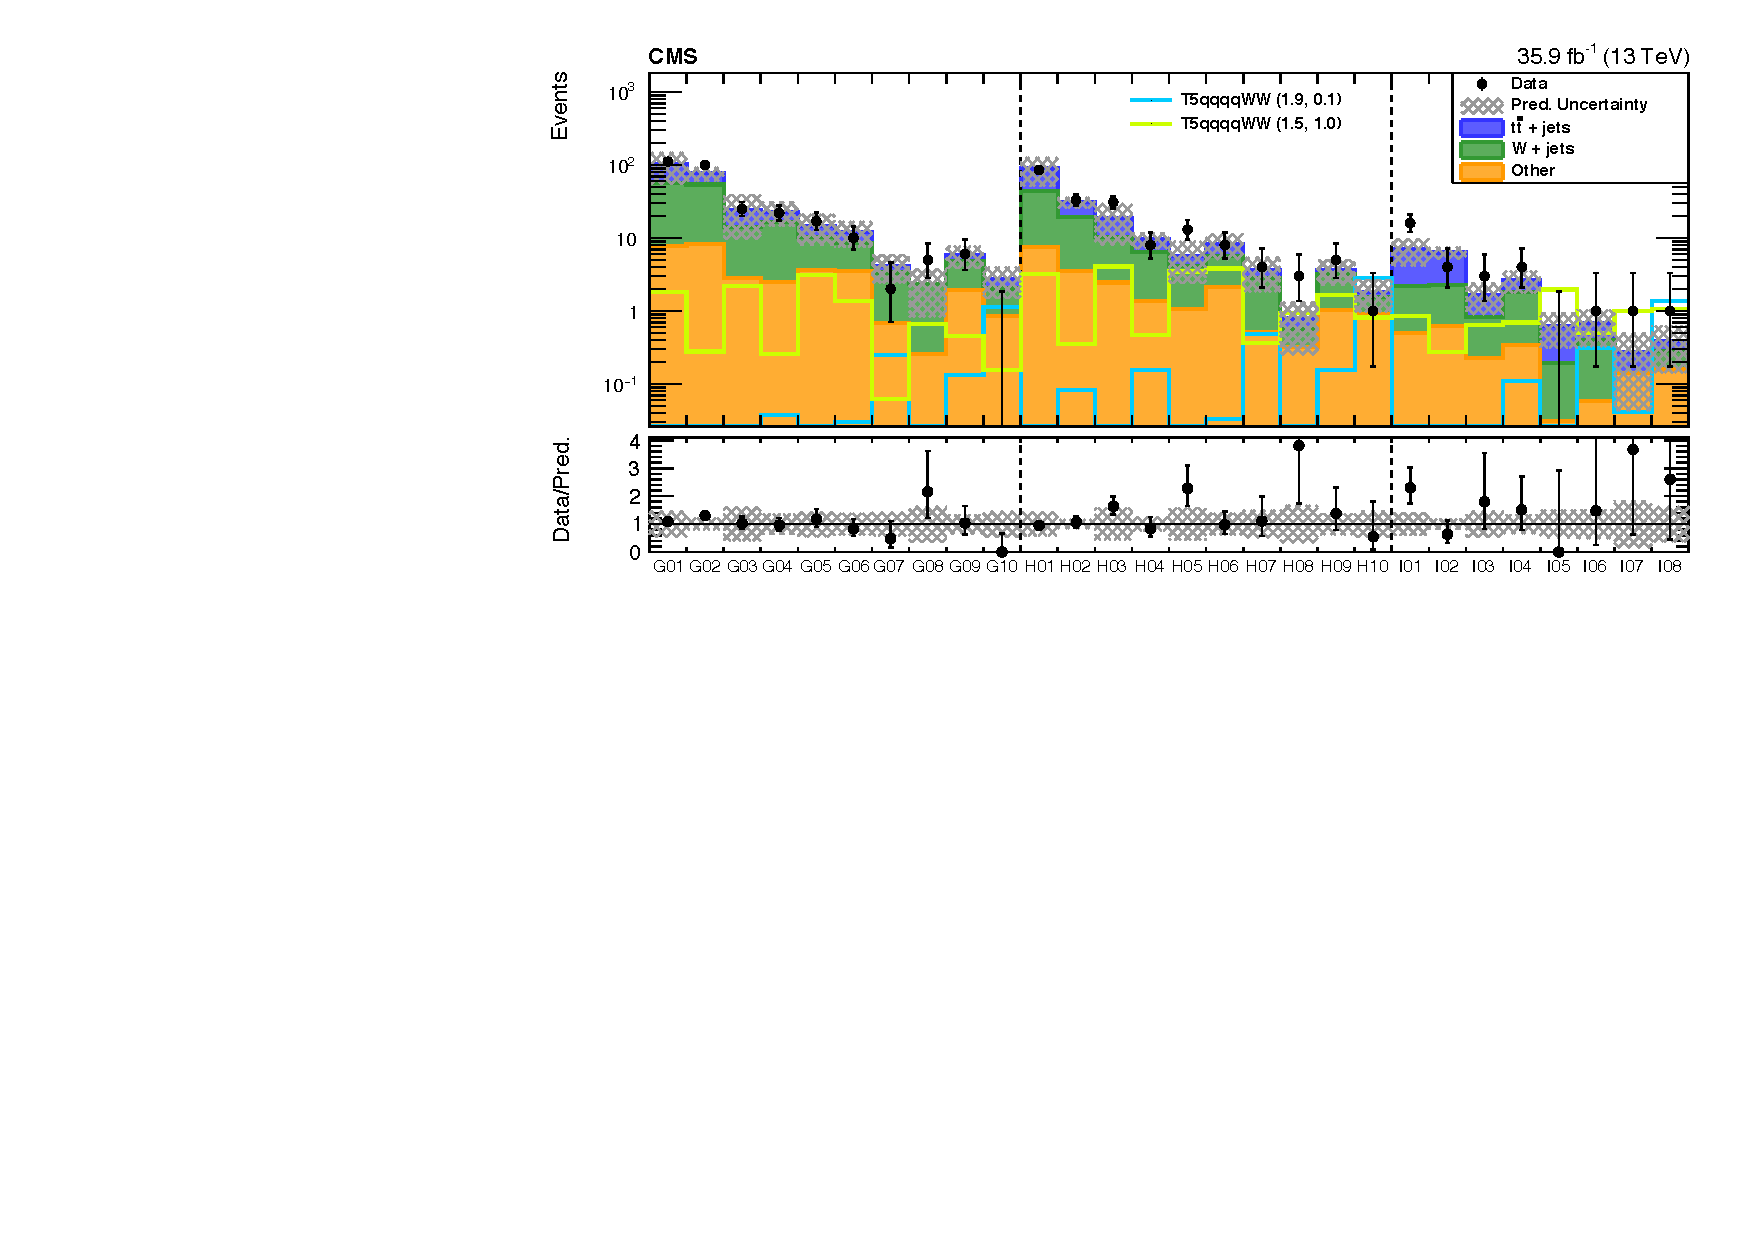
\includegraphics[width=0.9 \textwidth]{PhD_Thesis_v4/Plots/analysis/results/CMS-SUS-16-042_Figure_004.pdf}
    \caption[The results of main background estimation.]{Observed data and predicted event yields (from data) in the 28 search regions are shown. The black points with error bars show the number of observed data events and corresponding statistical error. The filled, stacked histograms represent the predictions for $\ttJets$, $\wJets$, and the remaining rare backgrounds. Lower panel shows the ratio of data to prediction and the shaded area reflects the total (stat. and syst.) relative uncertainty of the predicted background. 
    }
    \label{fig:mainRes}
\end{center}
\end{figure}
\begin{figure}[!h]
\begin{center}
    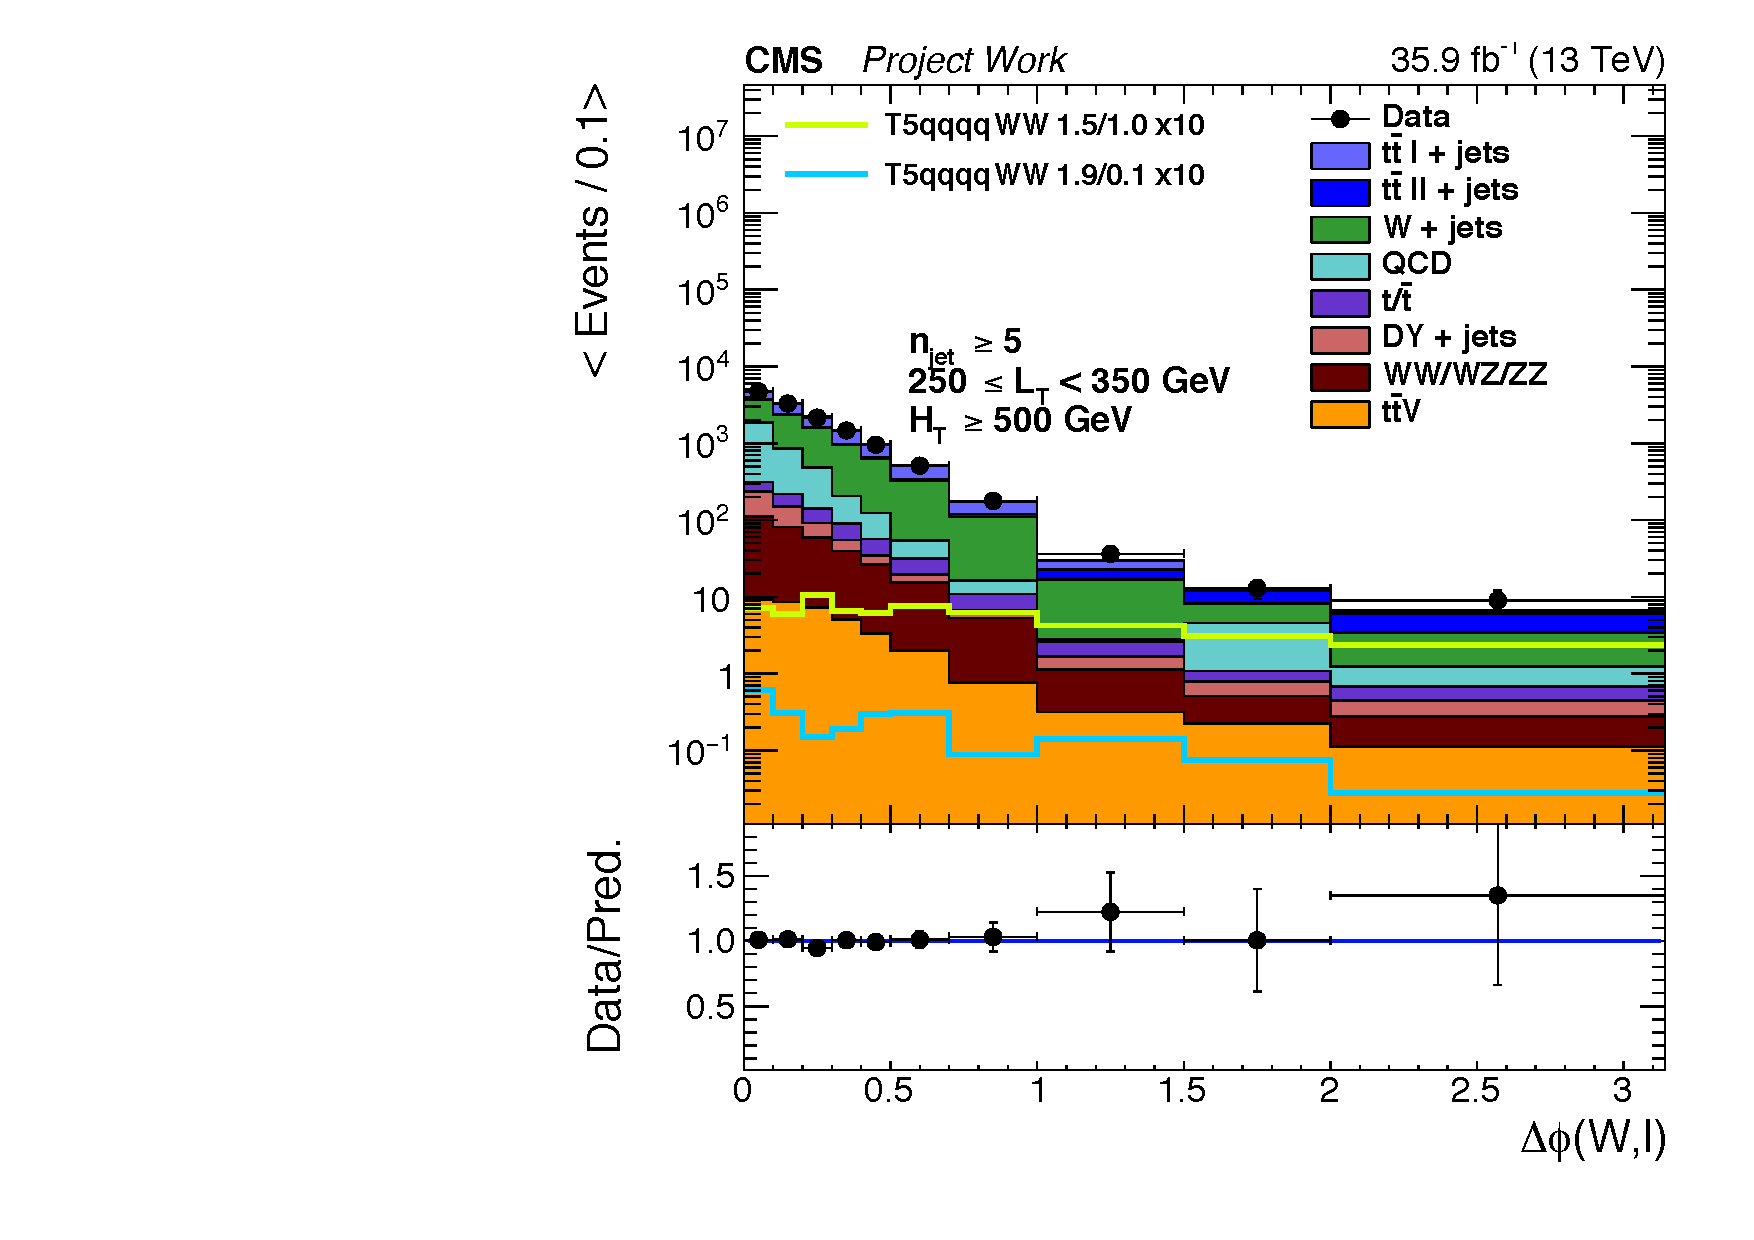
\includegraphics[width=0.45 \textwidth]{Plots/analysis/results/deltaPhi_Wl_wideProject1}
    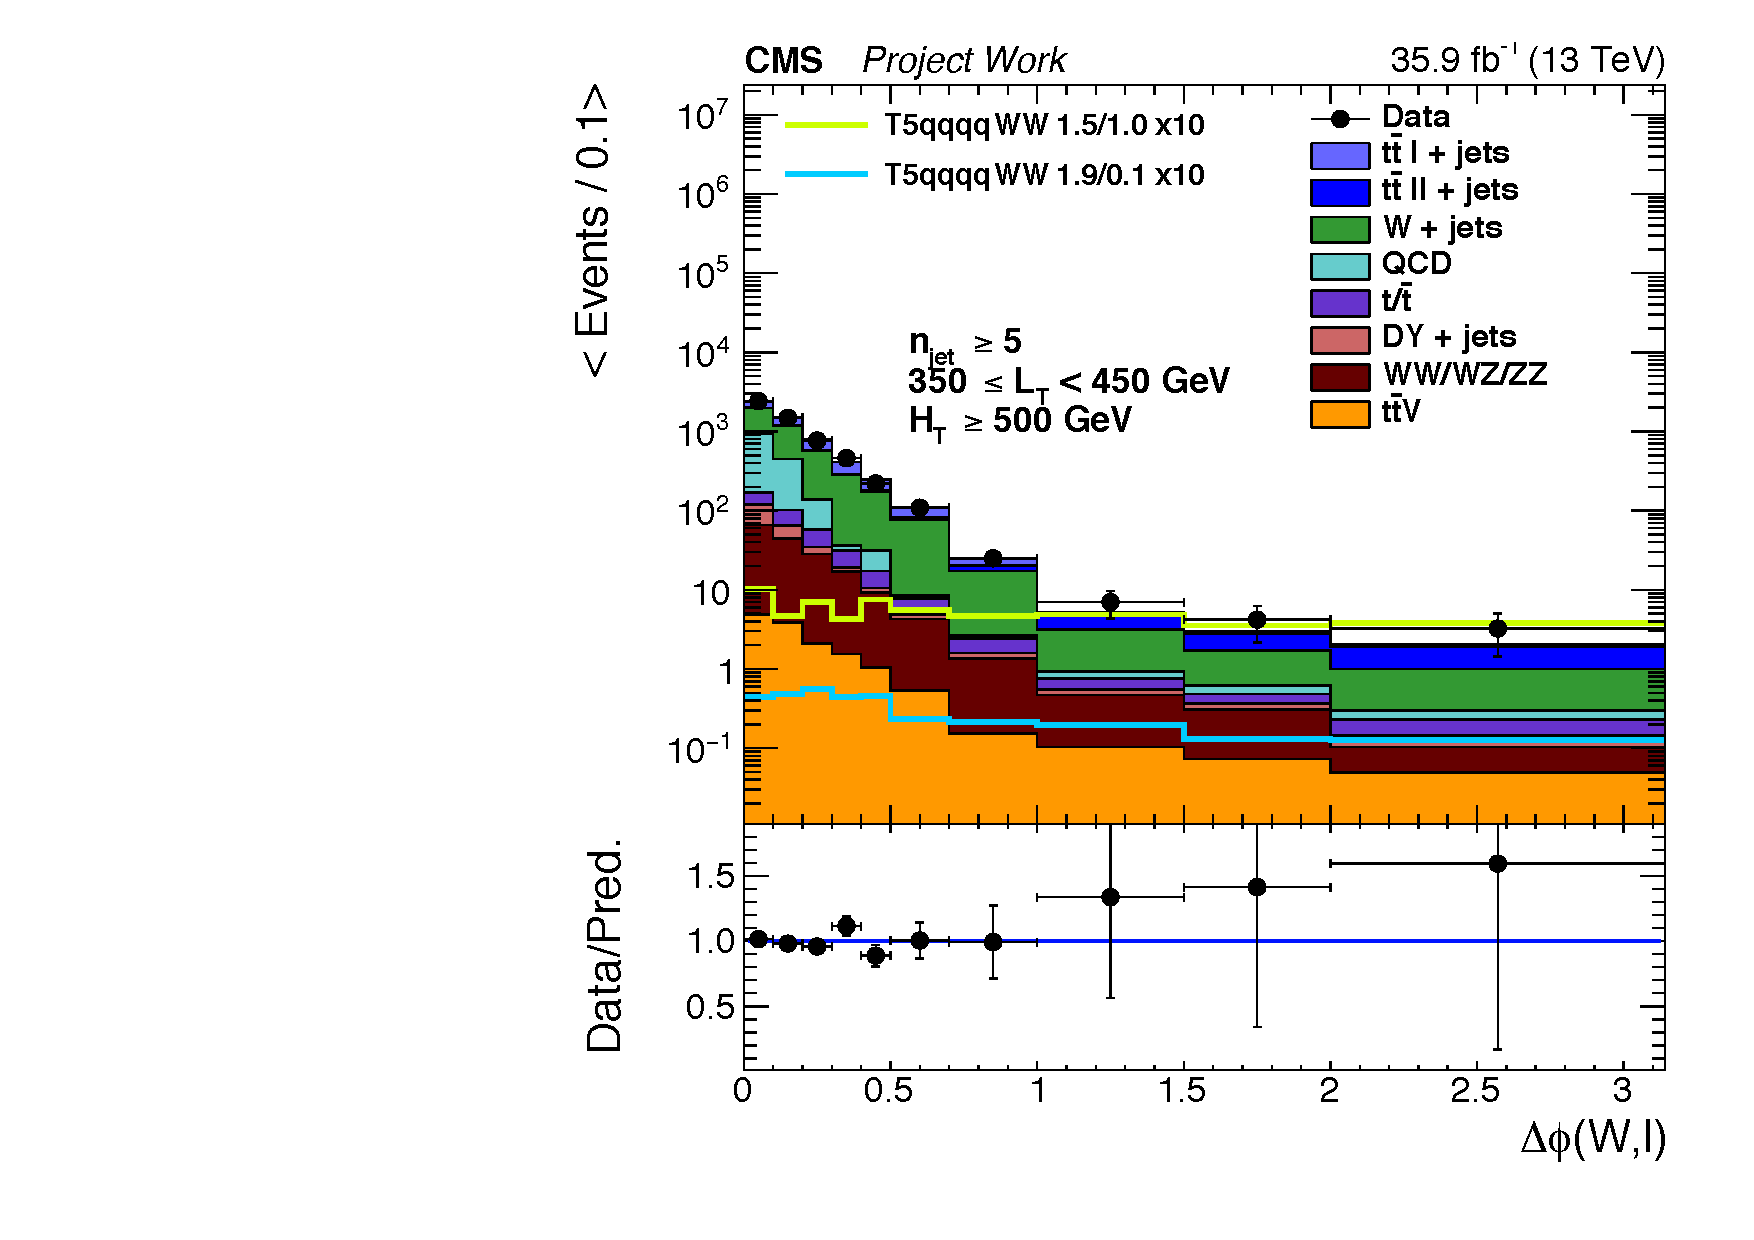
\includegraphics[width=0.45 \textwidth]{Plots/analysis/results/deltaPhi_Wl_wideProject2} \\
    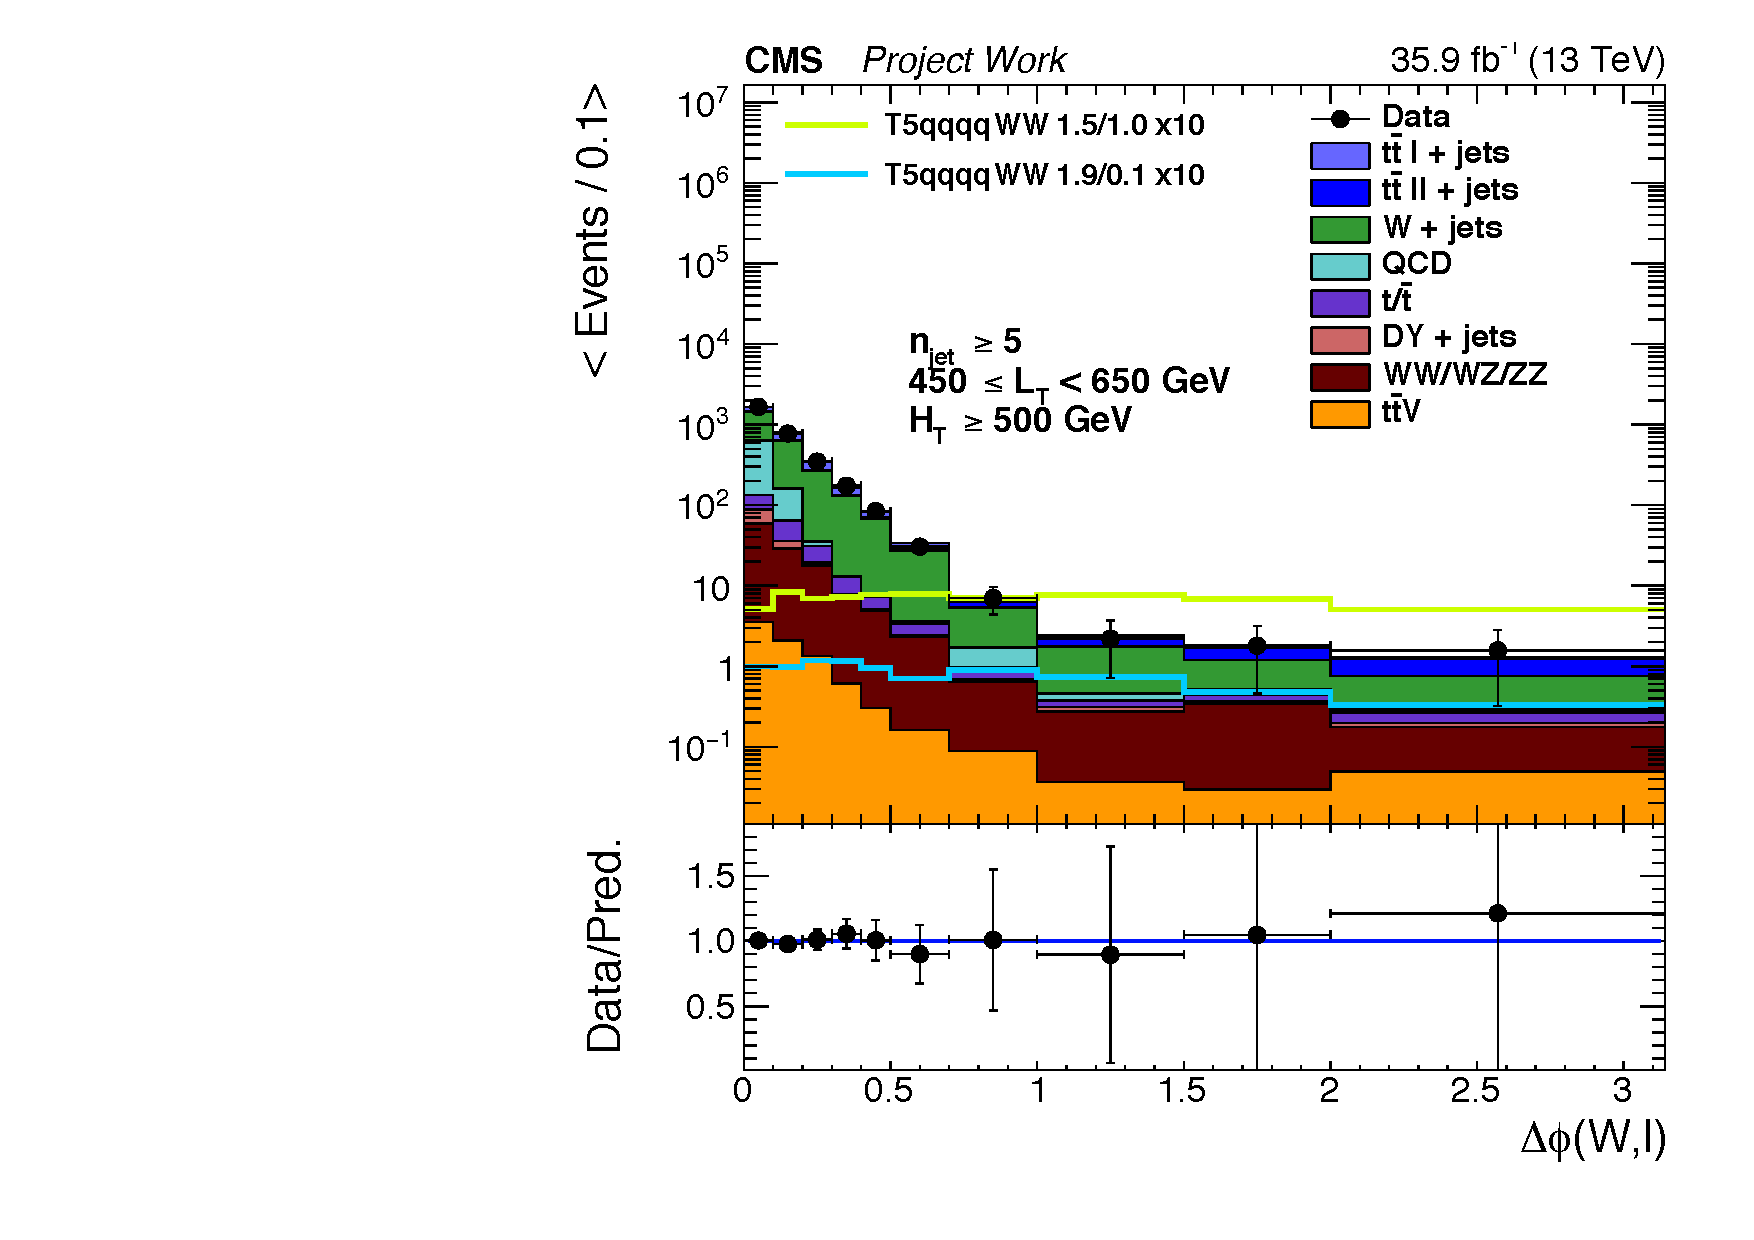
\includegraphics[width=0.45 \textwidth]{Plots/analysis/results/deltaPhi_Wl_wideProject3}
    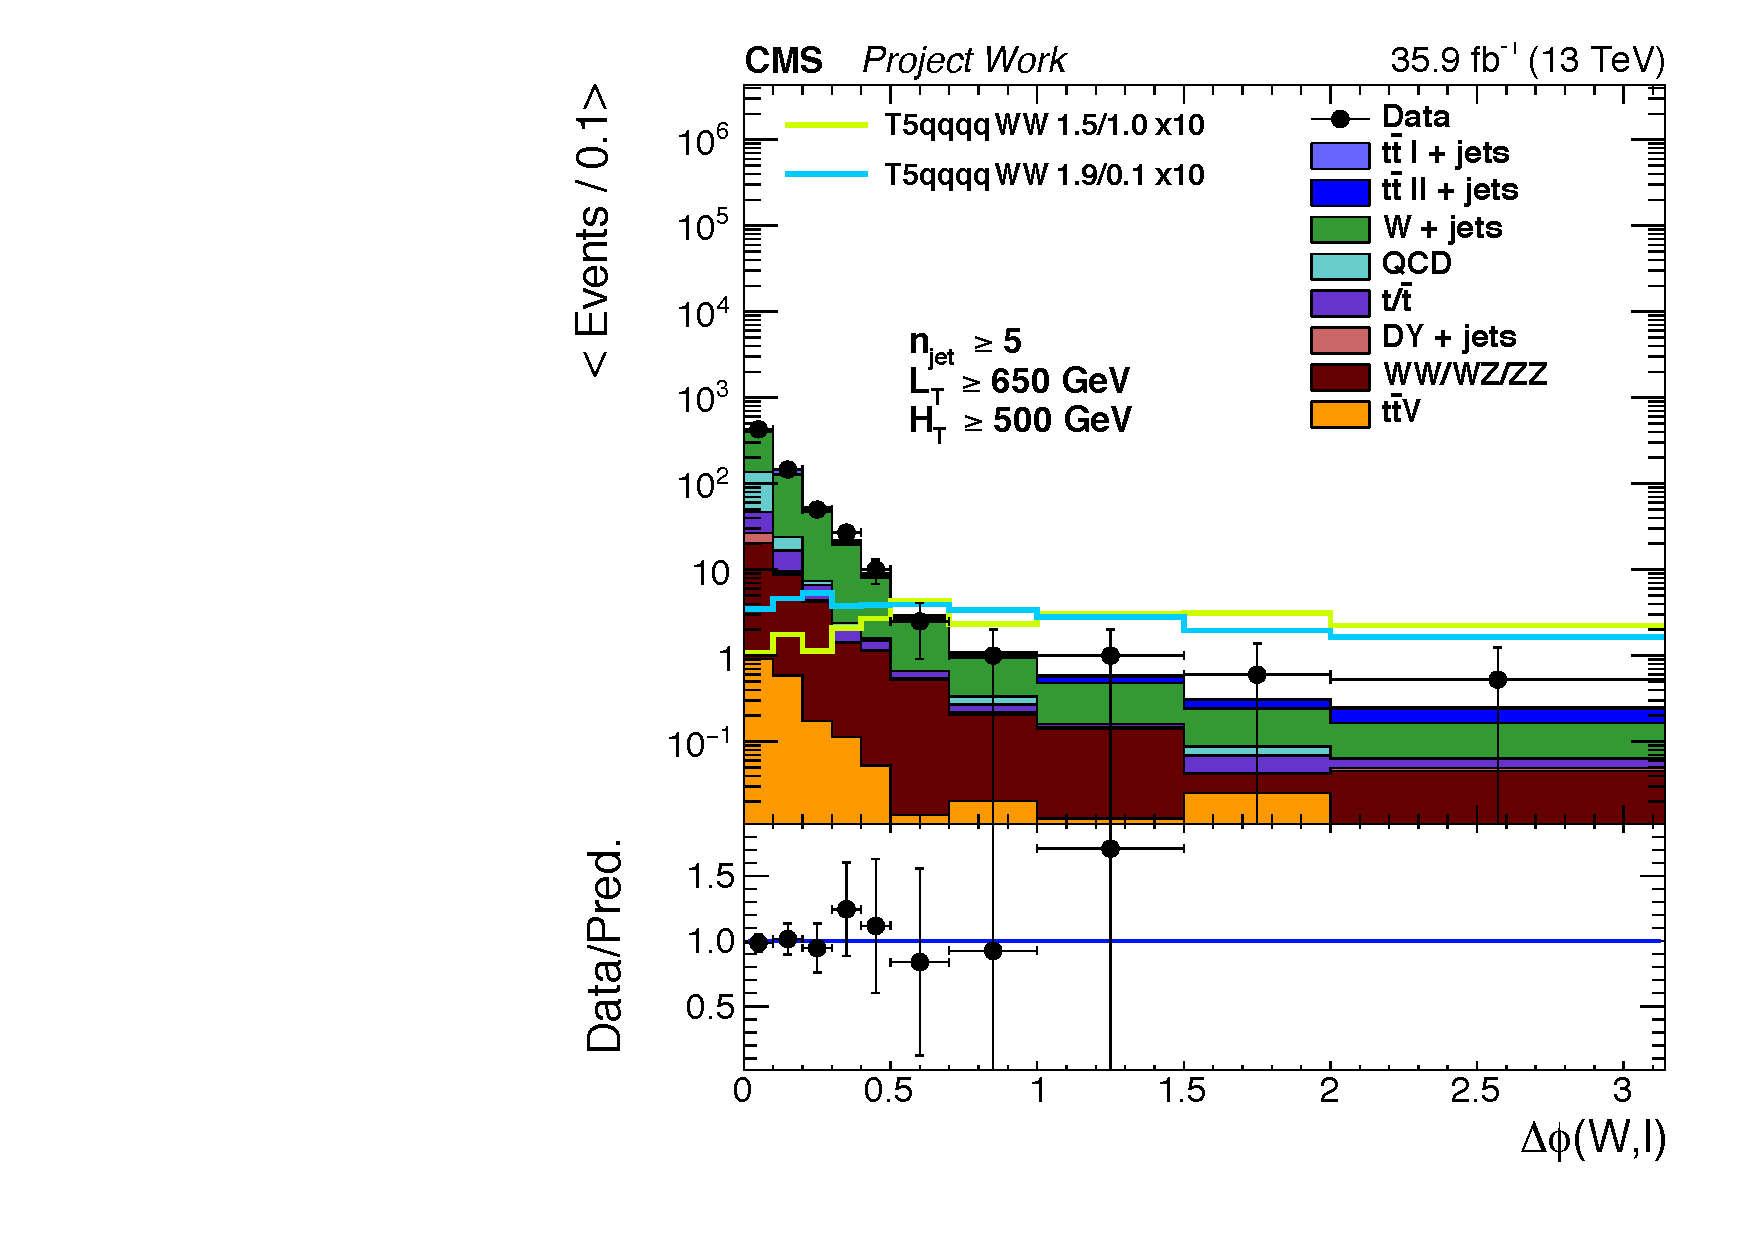
\includegraphics[width=0.45 \textwidth]{Plots/analysis/results/deltaPhi_Wl_wideProject4}
    \caption[The inclusive $\DF$ distributions]{$\DF$ distributions in data which is represented with black points and simulation which is represented with color filled areas. The figure shows the four $\LT$ interval after the baseline selection with inclusive requirements on $\njet\geq$ 5 and $\HT\geq$ 500 GeV. The simulated signal events are scaled by 10.
    }
    \label{fig:DFunblind}
\end{center}
\end{figure}
\subsection{Result of background prediction in aggregated regions}
\label{sec:AggrRes}
As mentioned in Sec.~\ref{sec:aggrSR}, 
 aggregate mainband signal regions have been defined to ease the reinterpretation of the results in terms future models.
 The comparison of the background predictions and the observed number of events in the SR of the aggregated SRs is presented in Tab.~\ref{tab:aggrRes}.
\begin{table}[!h]
\centering
\caption[The results of background estimation in aggregated regions.]{Numbers of expected background events with combined statistical
and systematic uncertainty and the observed numbers
of events in aggregated SRs. The expected number of signal
events for the two corresponding benchmark signals are given as well.}
\label{tab:aggrRes}\resizebox{\textwidth}{!}{
\begin{tabular}{c c c c c c c c}
 \njet  &  \LT & \DF & \HT & Pred. & Observed & T5qqqqWW & T5qqqqWW\\
  & [GeV] & [rad] & [GeV] & background & data & (1.5, 1.0)& (1.9, 0.1)  \\ \hline
 $\geq$ 5 &  $\geq$ 650 & 0.5  & $\geq$ 750 & 18.4 $\pm$ 5.1 &14 & 6.2$\pm$0.6 & 6.3$\pm$0.2 \\
 $\geq$ 6 &  $\geq$ 450 & 0.75  & $\geq$ 500 & 28.8$\pm$ 6.8&37 & 16.6$\pm$0.9 & 5.3$\pm$0.2\\
 $\geq$ 6 &  $\geq$ 650 & 0.5  & $\geq$ 1000 & 5.1$\pm$ 1.8&4 &  4.0$\pm$0.5 & 5.0 $\pm$0.2\\
 $\geq$ 7 &  $\geq$ 450 & 0.75  & $\geq$ 500 &  9.7$\pm$ 2.5&11 & 9.5$\pm$0.7 & 3.5$\pm$0.2\\
 $\geq$ 7 &  $\geq$ 650 & 0.5  & $\geq$ 500 & 3.8$\pm$ 1.2&4  & 4.3$\pm$0.5 & 3.3$\pm$0.2\\
 $\geq$ 8 &  $\geq$ 250 & 1.0  & $\geq$ 1250 & 7.2$\pm$ 1.9&8 & 1.8$\pm$0.3 & 1.7$\pm$0.1\\
\end{tabular}}
\end{table}
\newpage
\newpage
\newpage
\newpage
\newpage
\section{Statistical interpretation}
\label{LimitProc}
No significant excess is observed, and we proceed to upper limits on signal cross sections in the $m_{\tilde{g}}$-$m_{\ninozero}$ plane. In this section, the statistical framework used to derive limits is presented. The method includes not only the mainband signal regions (MB SR) but also sideband and control regions. For this purpose, a mechanism based on a statistical ABCD method where each letter is representing MB SR, MB CR, SB SR and SB CR respectively, is used. In this way, potential signal contamination in sideband and control regions is taken into account.
The limit procedure makes simultaneous use of two ABCD methods, called thus ABCDEF, since each of the $\ttJets$ and $\wJets$ backgrounds is predicted with two parallel but separate $\Rcs$ methods. A summary of these regions can be found in Tab.~\ref{tab:RCStoABCD}.
 \renewcommand{\arraystretch}{1.5}
\begin{table*}[!htb]
\caption{Conversion of $\Rcs$ regions to corresponding ABCDEF regions}
\label{tab:RCStoABCD}
\centering
\begin{tabular}{c|c|c}
                             & SR   & CR \\ \hline
MB & {\bf A} & B \\ \hline
$SB_{W}$      & C & D \\ \hline
 $SB_{\ttbar}$    & E & F \\
\end{tabular}
\end{table*}
\renewcommand{\arraystretch}{1.0}\\
The basic formulation of an ABCD method is shown in Eq.~\ref{tab:CLs1}, where QCD estimation is subtracted from CRs and possible residual differences between mainbands and sidebands are corrected with $\kappa$.
\begin{equation}
\label{tab:CLs1}
{\rm A}={\rm (B-B_{QCD})\,\cdot\,\frac{C}{(D-D_{QCD})}\,\cdot\,\kappa}.
\end{equation}
The formula representing the ABCDEF method is written as follows:
\begin{equation}
\label{tab:CLs2}
{\rm A}={\rm (B-B_{QCD})\,\cdot\,\,f_W\,\cdot\frac{C-C_{\ttbar}}{(D-D_{\ttbar})}\,\cdot\,\kappa_W\,\,+\,\, \rm (B-B_{QCD})\,\cdot\,f_{\ttbar}\,\cdot\, \frac{E}{(F-F_{QCD})}\,\cdot\,\kappa_{\ttbar}^{DL-corr}\,\cdot\, \kappa_{b} }.
\end{equation}
A tool that was developed for the search for the Higgs boson was used. This tool implements the statistical methods described in~\cite{CLs2}. The likelihood model has been extended to incorporate the ABCDEF regions and, specifically, the constraint described in Eq.~\ref{tab:CLs2}.
%As needed for the ABCD approach, for deriving the limits, the Higgs combination tool which is extended with a new functionality to handle non-linear relations between different regions, is used \cite{CLs2}.\\
Although taking a decision of setting limits is a Bayesian approach, the limit procedure for calculating exclusion curves and upper limits in the $\mgl$-$\mnone$ plane is based on the modified frequentist method. 
%After an introduction on the general statistical procedure for testing signal hypotheses and obtaining exclusion limits, the explanation of the implementation of these methods including the data-driven background estimation is discussed. At the end, upper limits on the cross section of the investigated SUSY models will be presented.
\subsection{Frequentist limit setting procedure}
In the frequentist approach, the goal is to find the probability to observe certain data under a given signal hypothesis.\\
%It is not to find the probability of that the signal model is true under the given observation. \\
Throughout this section, the expected event yields of SUSY model will be denoted as $s_i$, the SM background as $b_i$ where index "i" indicates corresponding MB. The systematic uncertainties are included as nuisance parameters $\theta$, such that signal and background predictions can be written as functions of the nuisances: $s_i(\theta)$ and $b_i(\theta)$. In the statistical treatment, all uncertainty sources are assumed to be either independent or 100\% correlated. The observed data events will be denoted as $data$. Finally, signal strength modifier is denoted as $\mu$. \\
\textbf{Likelihood function}\\
The likelihood function, which incorporates the ABCDEF regions for each mainband, is given by:
\begin{equation}
\label{likelihood}
  L = \prod^{ABCDEF}_i \textrm{Poisson}(data_i | b_i(\theta) + \mu \cdot s_i(\theta)) \times \prod^{\textrm{nuisances}}_j \textrm{Constraints}(\theta_j, \hat{\theta_j}),
\end{equation}
where the regions (A)BCDEF involves the Poisson p.d.f.s for the observed number of events given the (estimated)simulated sum of signal and background, and the second factor refers to the nuisance parameters. Both signal and background predictions are subject to multiple uncertainties. Systematic uncertainties which are discussed in Ch.~\ref{chapter:systematics} and $\kappa$ factors are included as constraints on the region A, while the QCD prediction is considered as constraints on the control regions B and F. Additionally, the nuisance parameters include the effect of the statistical uncertainty of all 6 bins.\\
The entire information is inserted to the limit tool using text files. An example text file is shown in Fig.~\ref{fig:datacard} for only one MB and moreover the entries corresponding to rare backgrounds and QCD have not been shown, for simplicity. Example tests on the nuisance parameters can be found in the Appendix~\ref{sec:nuisances} using the text file corresponding to the high mass gap benchmark point.
\begin{sidewaysfigure}
\begin{center}
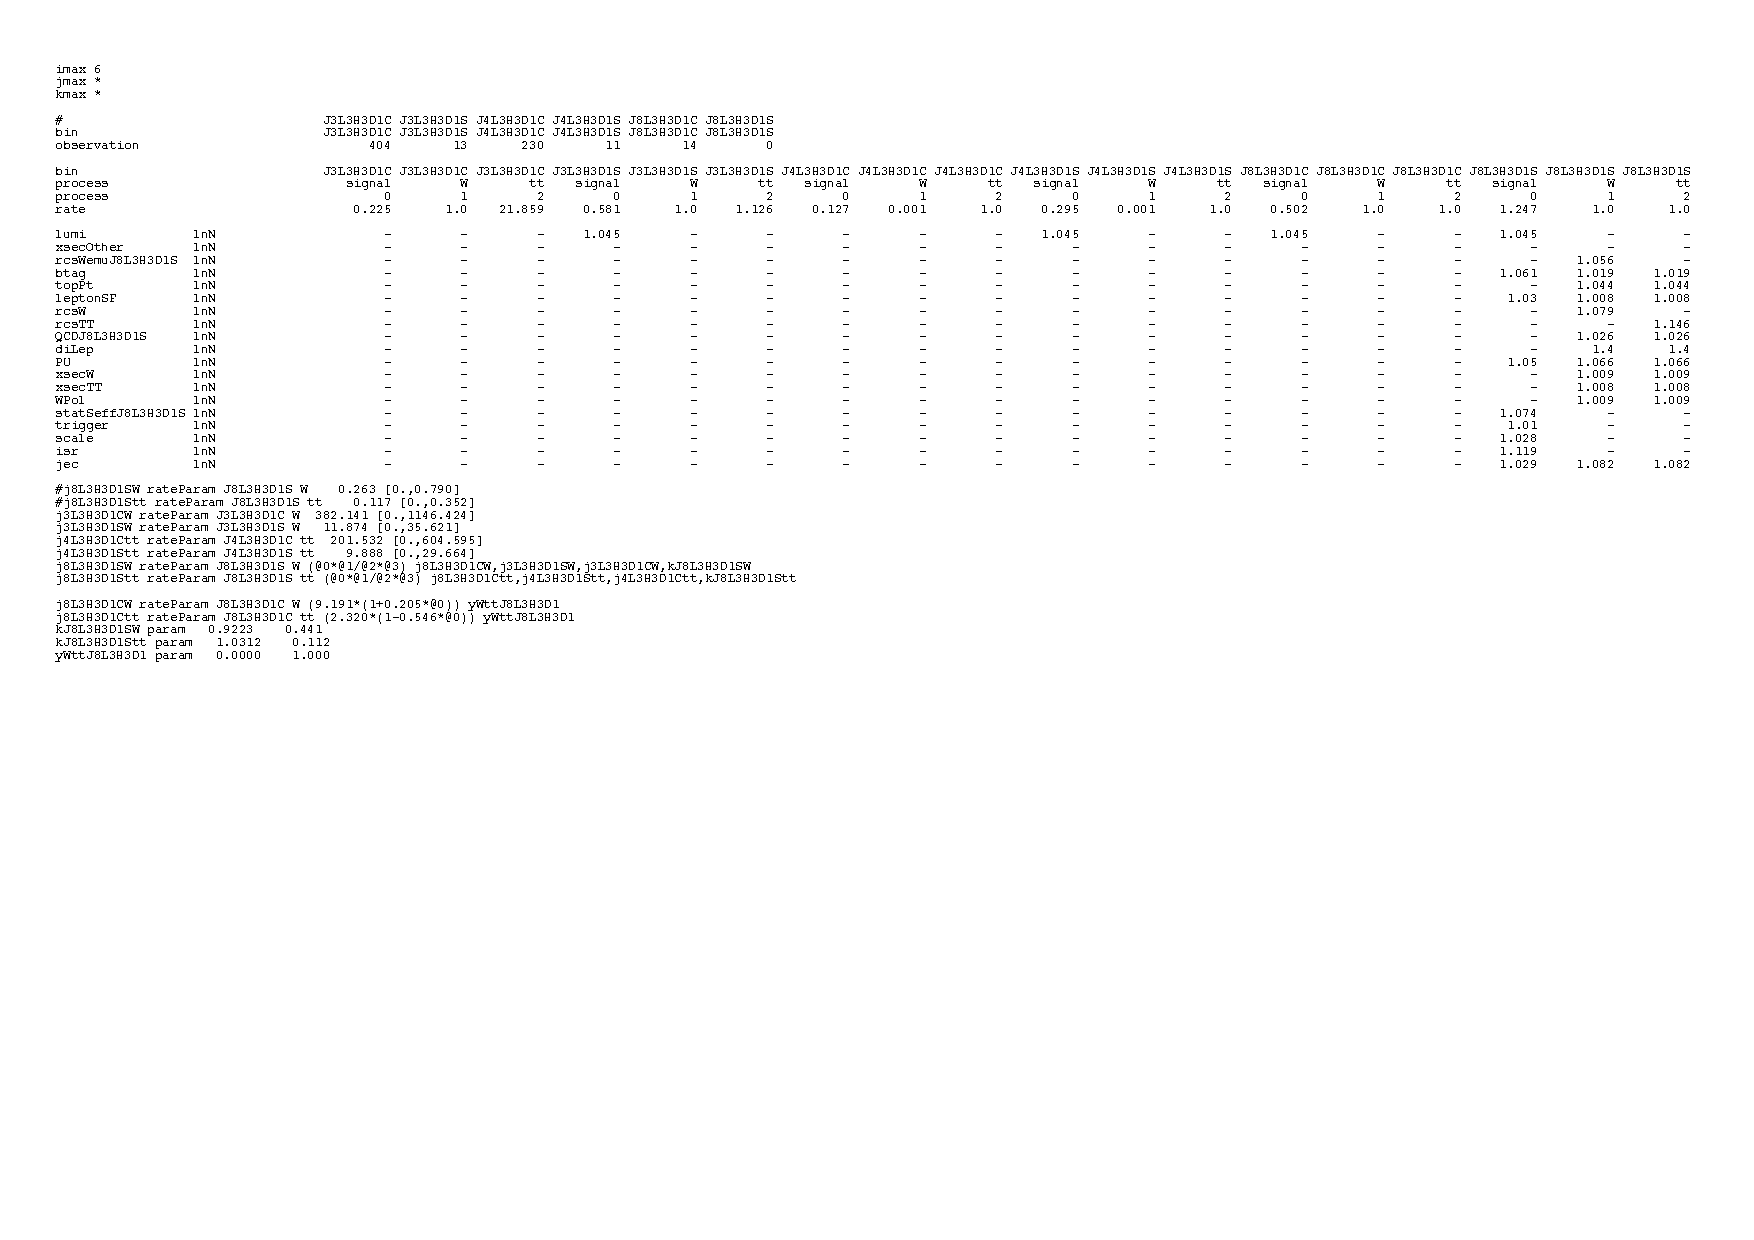
\includegraphics[width=\textwidth]{Plots/analysis/results/dataCardZeroB.pdf}
%\vspace{-5cm}
\caption{Simplified example of a text file file for one search region. 
The entries corresponding to rare backgrounds and QCD have been suppressed.}\label{fig:datacard}
\end{center}
\end{sidewaysfigure}
\\
%$\mu$ is the signal strength modifier and if it is 1 then signal+background hypothesis explains data well,  
\textbf{Test statistic, $\tilde{q}_{\mu}$}\\
The compatibility of the data with the background-only and signal+background
hypotheses, where the signal is allowed to be scaled by a factor $\mu$ is measured by constructing the
following test statistic based on the profile likelihood ratio \cite{CLs3}:
\begin{equation}
{\tilde{q}_\mu} = {-2\,{\rm ln}\frac{L(data|\mu,\, \hat{\theta}_{\mu})}{L(data|\hat{\mu},\, \hat{\theta})}}, \,\,\,\, for \,\,\,\, 0 \leq\hat{\mu}\leq\mu,
\end{equation}
where nominator and denominator are maximized separately. $\hat{\theta}_{\mu}$ is the conditional maximum given the signal strength modifier value $\mu$. $\hat{\mu}$ and $\hat{\theta}$ are corresponding to the global maximum of the likelihood. $\hat{\mu}$ and $\hat{\theta}$ are free parameters so the denominator is independent of $\mu$ and serves as a normalization term only. The condition $0\leq\hat{\mu}\leq\mu$ ensures one-sided confidence intervals for upper limit tests while nonphysical negative signals are avoided.\\
According to the Neyman-Pearson lemma \cite{Lemma}, the ratio of likelihoods provide the most powerful discrimination. However, this statement does not have to be true for a system with multiple free parameters, in fact the existence of a uniformly most powerful test statistic is not certain. On the other hand, the likelihood ratio has proven reliable and is easy to use. Therefore, it is commonly used in experimental particle physics.
\\
\textbf{Observed $\tilde{q}_{\mu,\,\rm obs}$ and $\hat{\theta}_{\mu,\,\rm obs}$}\\
The observed value of the test statistic ($\tilde{q}_{\mu,\,\rm obs}$) and the nuisance parameter ($\hat{\theta}_{\mu,\,\rm obs}$)  for a given signal strength $\mu$ that maximize the likelihood function given in Eq.~\ref{likelihood} are computed.
The case of $\mu=0$ corresponds to the background-only hypothesis while the non-zero $\mu$ values are representing the signal+background hypothesis.\\
%If one finds good agreement with data with a large $\mu$, it would probably mean new physics. \\
\textbf{Pdfs $\tilde{q}_{\mu}$}\\
To compute the test statistic pdfs $p_{\mu}$($\tilde{q}_{\mu}|\mu,\,\hat{\theta}_{\mu}$), generation of toy pseudo-MC samples with a signal strength of $\mu$ and $\mu=0$ is in principle required. This procedure requires to scan a range of $\mu$ values and subsequently generate a large number of pseudo-experiments. However, in the present complex case, the pseudo-MC mechanism is prohibitively computationally expensive. Therefore, asymptotic formulae~\cite{asymtForm} are used to circumvent this computational challenge.\\ 
%The procedure involves usage of analytic formulas instead of toy MC.\\
\textbf{Observed p-value for hypothesis $\mu$}\\
The observed p-value for hypothesis $\mu$ can be calculated as:
\begin{equation}
\label{p-value}
  P(\mu) = \int_{\tilde{q}_{\mu,\,\rm obs}}^{\infty} p_{\mu}(\tilde{q}_{\mu} | \mu,\,\hat{\theta}_{\mu}) d_{{\tilde q}_{\mu}}.
\end{equation}
The probability of finding a value of test under the background only hypothesis at least as large as the one observed in data, $P(q_0\geq q_{0,\rm obs})$, can be used in quantifying an excess.\\
The p-value can be converted into significance by through one-sided normal distribution tail probability:
\begin{equation}
\label{sig_pval}
  P = \int_{Z}^{\infty} \frac{1}{\sqrt{2\pi}}exp(-x^2/2) d_x.
\end{equation}
The asymptotic approximation mentioned above allows to estimate the significance, $Z$ in Eq.~ \ref{sig_pval}, directly from the observed test systematic as:
\begin{equation}
  {Z} = {\sqrt{q_{0,\rm obs}}}.
\end{equation}
This is possible, because the profile likelihood test statistic is distributed as a $\chi^2$ distribution with one degree of freedom~\cite{halfChiSq}. In particle physics, to claim "discovery", the significance must exceed Z=5, which is corresponding to a one-sided p-value of the back-ground only hypothesis of 2.87$\cdot$10$^{\rm -7}$. The observed significance, which is obtained by combining the main search regions,  for the signal model T5qqqqWW is presented in Fig. \ref{fig:obsig}. It can be seen that for all the mass points the local significance is less than 3.\\
\begin{figure}[!h]
\begin{center}
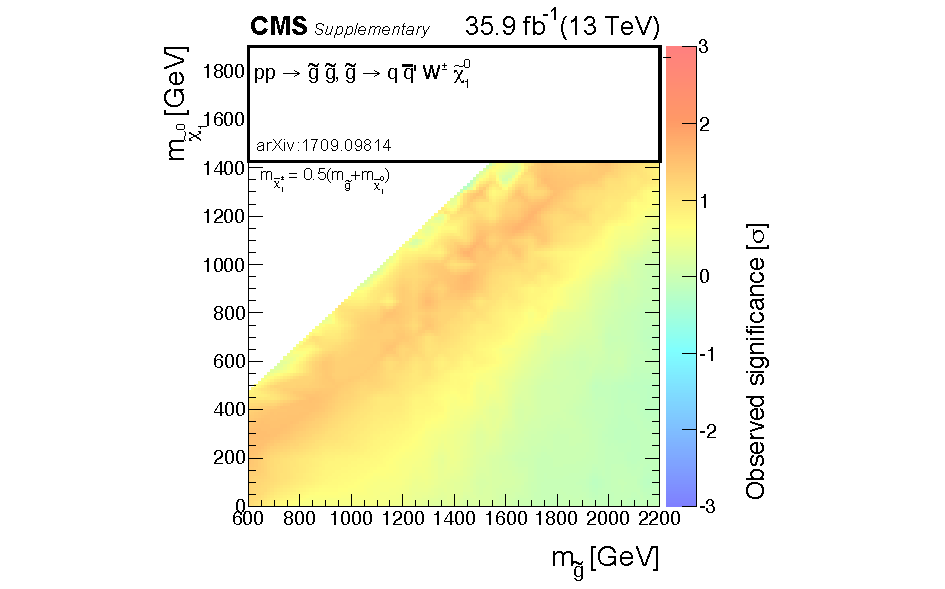
\includegraphics[width=0.8\textwidth]{Plots/analysis/results/CMS-SUS-16-042_Figure-aux_002.pdf}
%\vspace{-5cm}
\caption{Observed significance for the model T5qqqqWW.}\label{fig:obsig}
\end{center}
\end{figure}
\textbf{Upper limits}\\
Upper limits are calculated at the 95\% confidence level(CL) using the asymptotic CL$_{\rm s}$ criterion~\cite{CLs1}, where CL$_{\rm s}$ is defined as:
 \begin{equation}
\label{uplim}
  CL_{\rm s}=\frac{CL_{\rm s+b}}{CL_{\rm b}}.
\end{equation}
$CL_{\rm s+b}$ can be constructed using the probability of finding a value of $q_\mu$ at least as larger as the observed one under the signal+background hypothesis, $P(q_0\geq q_{0,\rm obs}|\mu)$, while $CL_{\rm b}$ can be constructed using the background only hypothesis, $P(q_0\geq q_{0,\rm obs}|\mu=0)$.
The 95\% CL exclusion limits are defined as $CL_{\rm s}$$(\mu)\leq5$\%.\\

Given the fact that the ratio is also sensitive to downwards fluctuations of the background, this condition is more conservative than only considering signal+background hypothesis, i.e $CL_{\rm s+b}(\mu)\leq5$.  
Finally, $\mu$ is varied iteratively until  $CL_{\rm s}=5$\% and if $\mu$ is smaller than 1, a signal mass scenario is excluded.
%The confidence level expression, which is abbreviated shortly by CL \cite{CLs2}, represents incompatibility of a signal hypothesis with data. \\
 %and a signal is excluded if $\mu$ is smaller than one. Requiring 95\% CL leads that limit on $\mu$ approaches to one, it is, however, a conventional choice in high-energy physics.
%The modified frequentist method, often referred to as CLs, is used to obtain limits \cite{CLs1}. The LHC Higgs Combination Group including members of the ATLAS and CMS collaboration refined the method for combining search regions for the Higgs search results \cite{CLs2}.
\section{Interpretation on simplified model T5qqqqWW}
As discussed earlier, the supersymmetric simplified models (see Sec.~\ref{sec:simplifiedModels}) are used to interpret the results of the search. Because of the absence of any significant deviation from the data-based SM prediction, upper limits  on the cross section of the T5qqqqWW model are derived in the mass plane.  
The procedure introduced in Sec.~\ref{LimitProc} is followed to obtain 95\% CL upper limits on the observed and the median expected signal strength. The corresponding results are presented in Fig.~\ref{fig:uplims} for the entire mass scan of the T5qqqqWW. The values for the missing mass points, that can be seen in Fig.~\ref{fig:massplane}, are compensated by interpolating between the neighboring $\mu$ values.
The upper limit on the production cross section of the T5qqqqWW model can be obtained by multiplying the upper limit obtained on signal strength $\mu$ with the theoretical cross section.
In Fig.~\ref{fig:FinalLim}, the color map shows the observed upper limit on the theoretical cross section, the black lines show the corresponding exclusion curve and $\pm$1$\sigma$ contours due to theoretical uncertainty on cross section. In the same figure, the red lines are the expected exclusion limit contours. \\
%The simplified model T5qqqqWW, which contains gluino pair production with the gluinos decaying to first- or second-generation squarks and a chargino, which subsequently decays to
%a W boson and the lightest neutralino. 
In the region where the mass difference between gluino and neutralino is high, the decay products typically have high momenta. Therefore, kinematic regions with high hadronic and leptonic scales provide the largest signal sensitivity. In this region, the observed limit follows the expected median and the T5qqqqWW simplified model scenarios with gluino mass up to~1.9~TeV for neutralino masses below~300~GeV  are excluded. \\
In the region close to compressed mass scenarios, where the gluino has very soft decay products resulting in a decrease in acceptance, the upper limit on the cross section takes values up to~1~pb. The signal  models with neutralino mass up to~950~GeV are excluded.
To investigate the reason why the observed limit curve is significantly below the expected one a benchmark point with gluino mass~1.4~TeV and neutralino mass~1~TeV is chosen. It is found to be that the most sensitive bin which is $\njet \leq 8$, $450\leq\LT<650$~GeV, $500\leq\HT<1250$~GeV does not show an excess. However, there are 6 bins with a similar sensitivity out of which three show light excesses. Especially, the bin with $6\leq\njet\leq7$, $450\leq\LT<650$~GeV, $500\leq\HT<750$~GeV has~13~events observed while 5.7$\pm$3.3 expected.
\begin{figure*}[!h]
\centering
  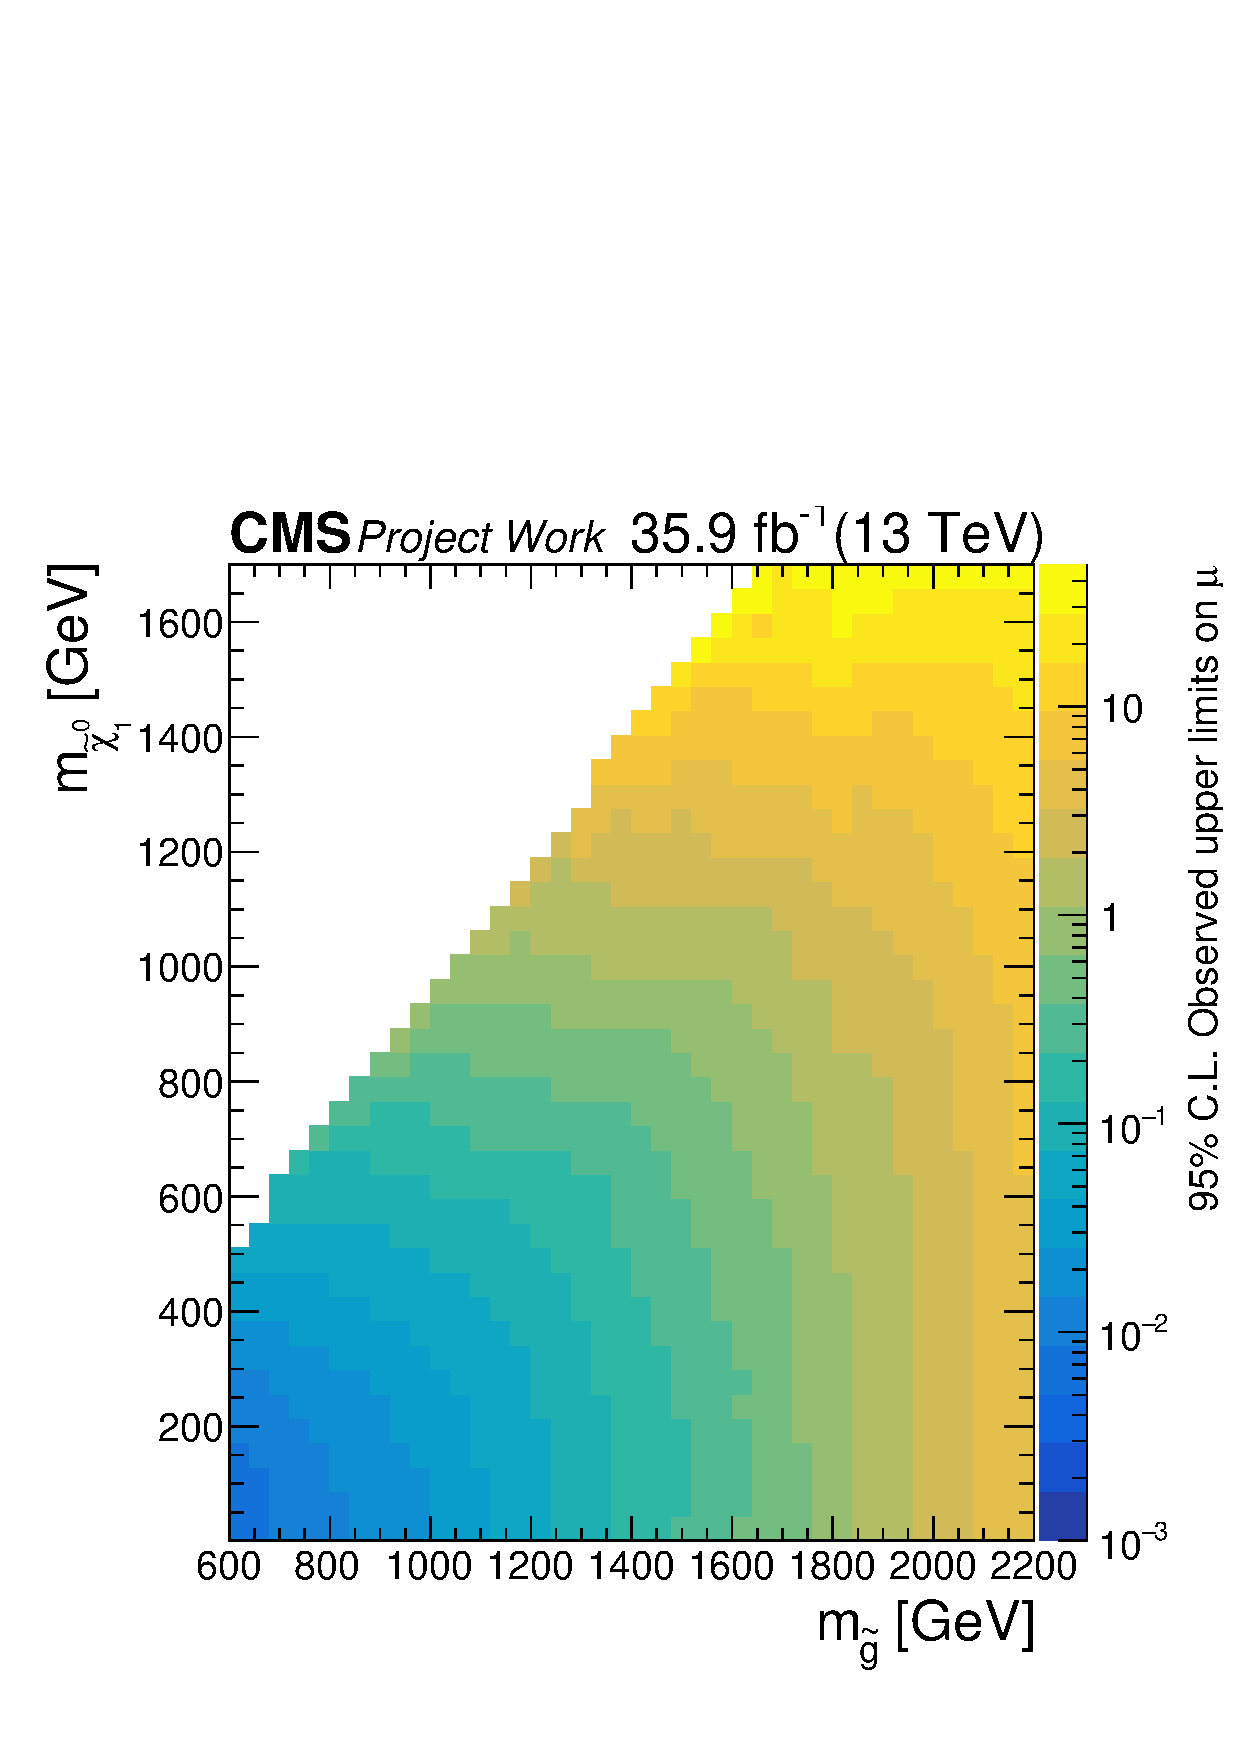
\includegraphics[width=0.45\textwidth]{PhD_Thesis_v4/Plots/analysis/results/ObsLimNew.pdf}
 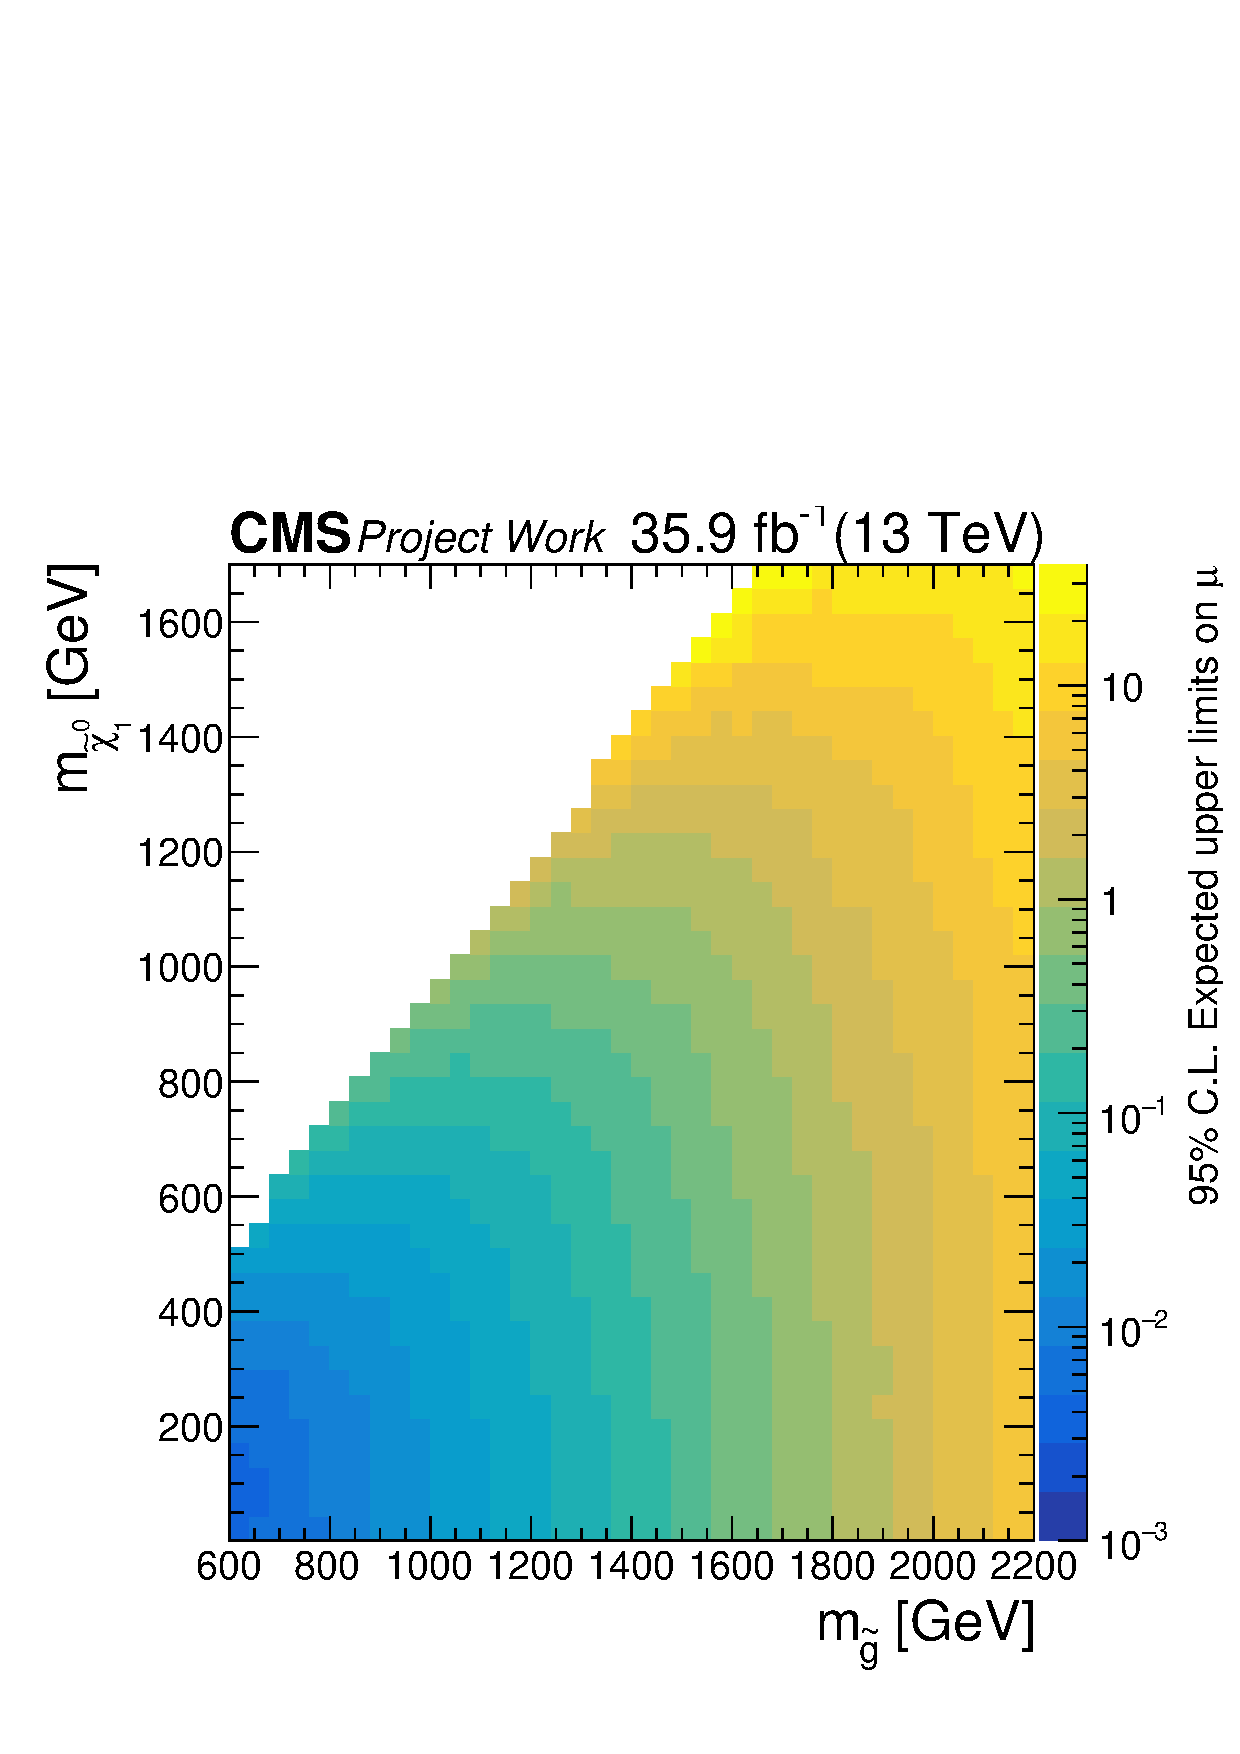
\includegraphics[width=0.45\textwidth]{PhD_Thesis_v4/Plots/analysis/results/ExpLimNew.pdf}
  \caption{ 95\% CL Observed (Expected) upper limits on the signal strength modifier $\mu$ for the T5qqqqWW model is shown at the left (right) side as a function of the gluino and neutralino masses.
  }
  \label{fig:uplims}
\end{figure*}

\begin{figure*}[!h]
\centering
  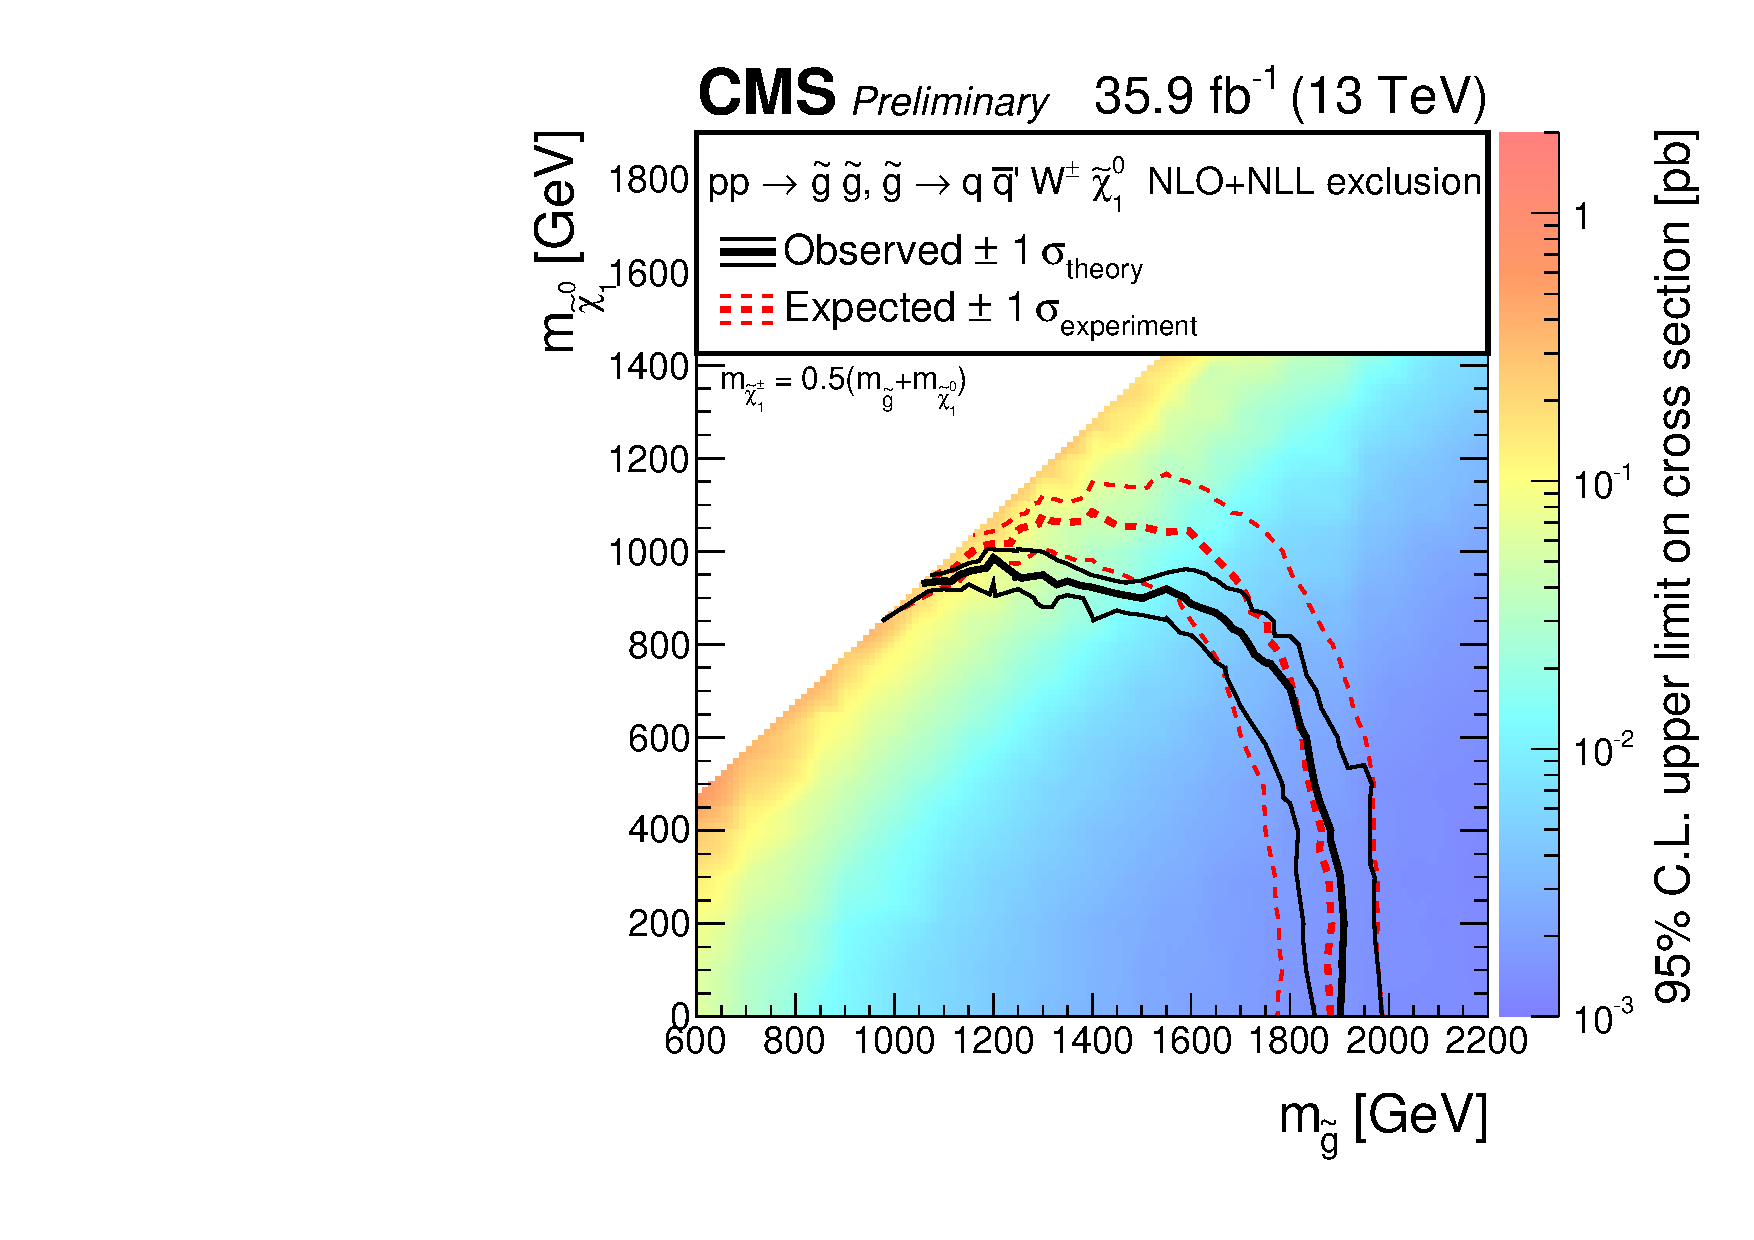
\includegraphics[width=0.6\textwidth]{Plots/analysis/results/CMS-PAS-SUS-16-042_Figure_004-b.pdf}
  \caption{ Cross section limits at a 95\% CL for the T5qqqqWW model, and as a function of the gluino and LSP masses. The solid black (dashed red) lines correspond to the observed (expected) mass limits, with the
  thicker lines representing the central values and the thinner lines
representing the $\pm 1\sigma$ uncertainty bands related to the theoretical
(experimental) uncertainties
  }
  \label{fig:FinalLim}
\end{figure*}

\section{Comparison to complementary results}
\label{sec:Comparison}
As discussed in Sec.~\ref{sec:histSus}, the simplified SUSY model T5qqqqWW had already been studied in Run1 of LHC and the models with gluino mass up to~900~GeV were excluded~\cite{SUSRun1}. The searches are repeated at the new center-of-mass energy and the first results were published with integrated luminosity of~2.3~fb$^{-1}$~\cite{SUS_16_005}. In the present analysis, the exclusion on the gluino mass is extended by~500~GeV for the lowest neutralino mass.\\
The results of new Run~2 analyses of CMS with 35.9~fb$^{-1}$ are shown in the left plot of Fig.~\ref{fig:SUSY_strong_1step}. The present analysis, which is labeled with SUS-16-042, is represented with the purple curve and published in~\cite{SUS_16_042}. The analysis covers the largest area in the high gluino-neutralino mass gap while another analysis, which is labeled with SUS-16-033~\cite{SUS_16_033}, covers the largest area in the region close to compressed scenarios. This second analysis performs a search in the full-hadronic final state, where both of the W bosons decay hadronically, using the missing $\HT$ variable. The missing $\HT$ is calculated very similar to the $\MET$ but using only the the transverse momentum of jets.\\
An overall summary of the SUSY results analyzed by CMS can be found at the bottom plot of the Fig.~\ref{fig:susy_Summary}. Figure shows the best exclusion limits on sparticle masses. Almost all the analyses, which set limits on gluino mass, have competitive results reaching up to~2~TeV. \\
The ATLAS collaboration performed also several searches for gluino pair production. The results for the topologies similar to the T5qqqqWW of CMS can be seen in Fig.~\ref{fig:SUSY_strong_1step}~(right) where the gray shaded area shows the Run~1 results. Furthermore, a summary of all SUSY models studied in ATLAS is shown  in Fig.~\ref{fig:susy_Summary}~(top). \\

\begin{figure*}[!hb]
\centering
  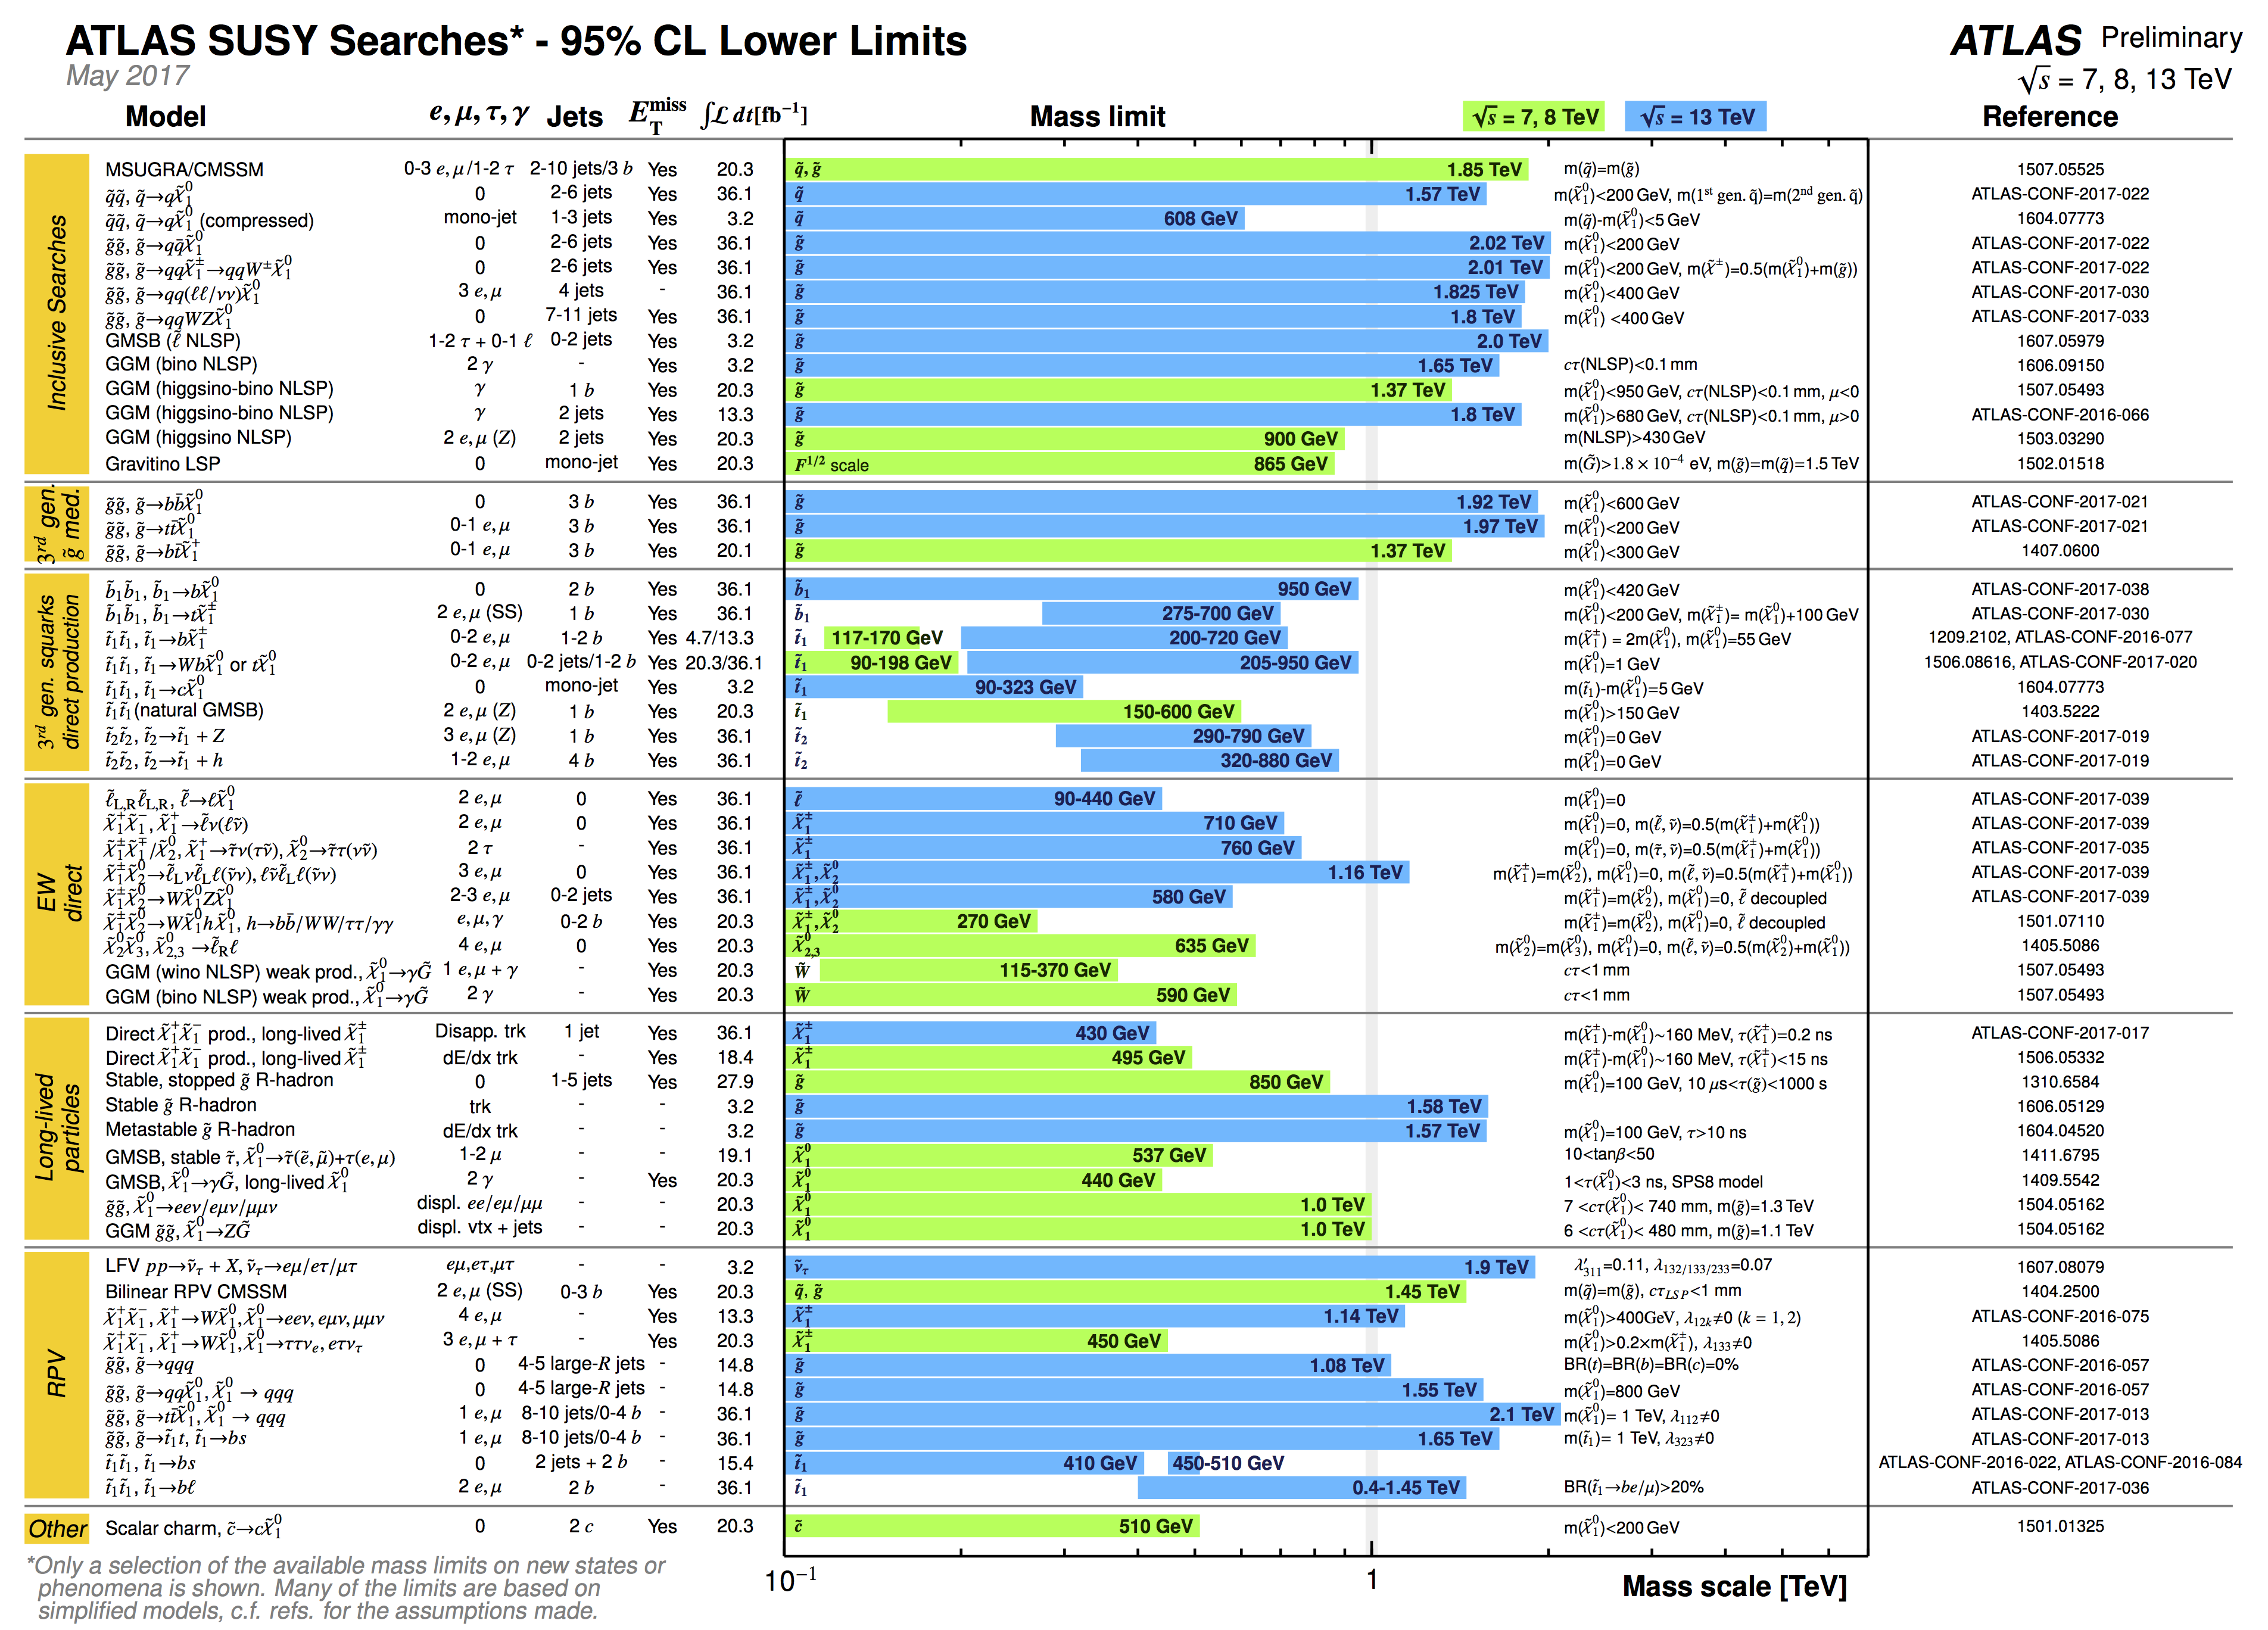
\includegraphics[width=0.9\textwidth]{Plots/SUSY/ATLAS_SUSY_Summary}
  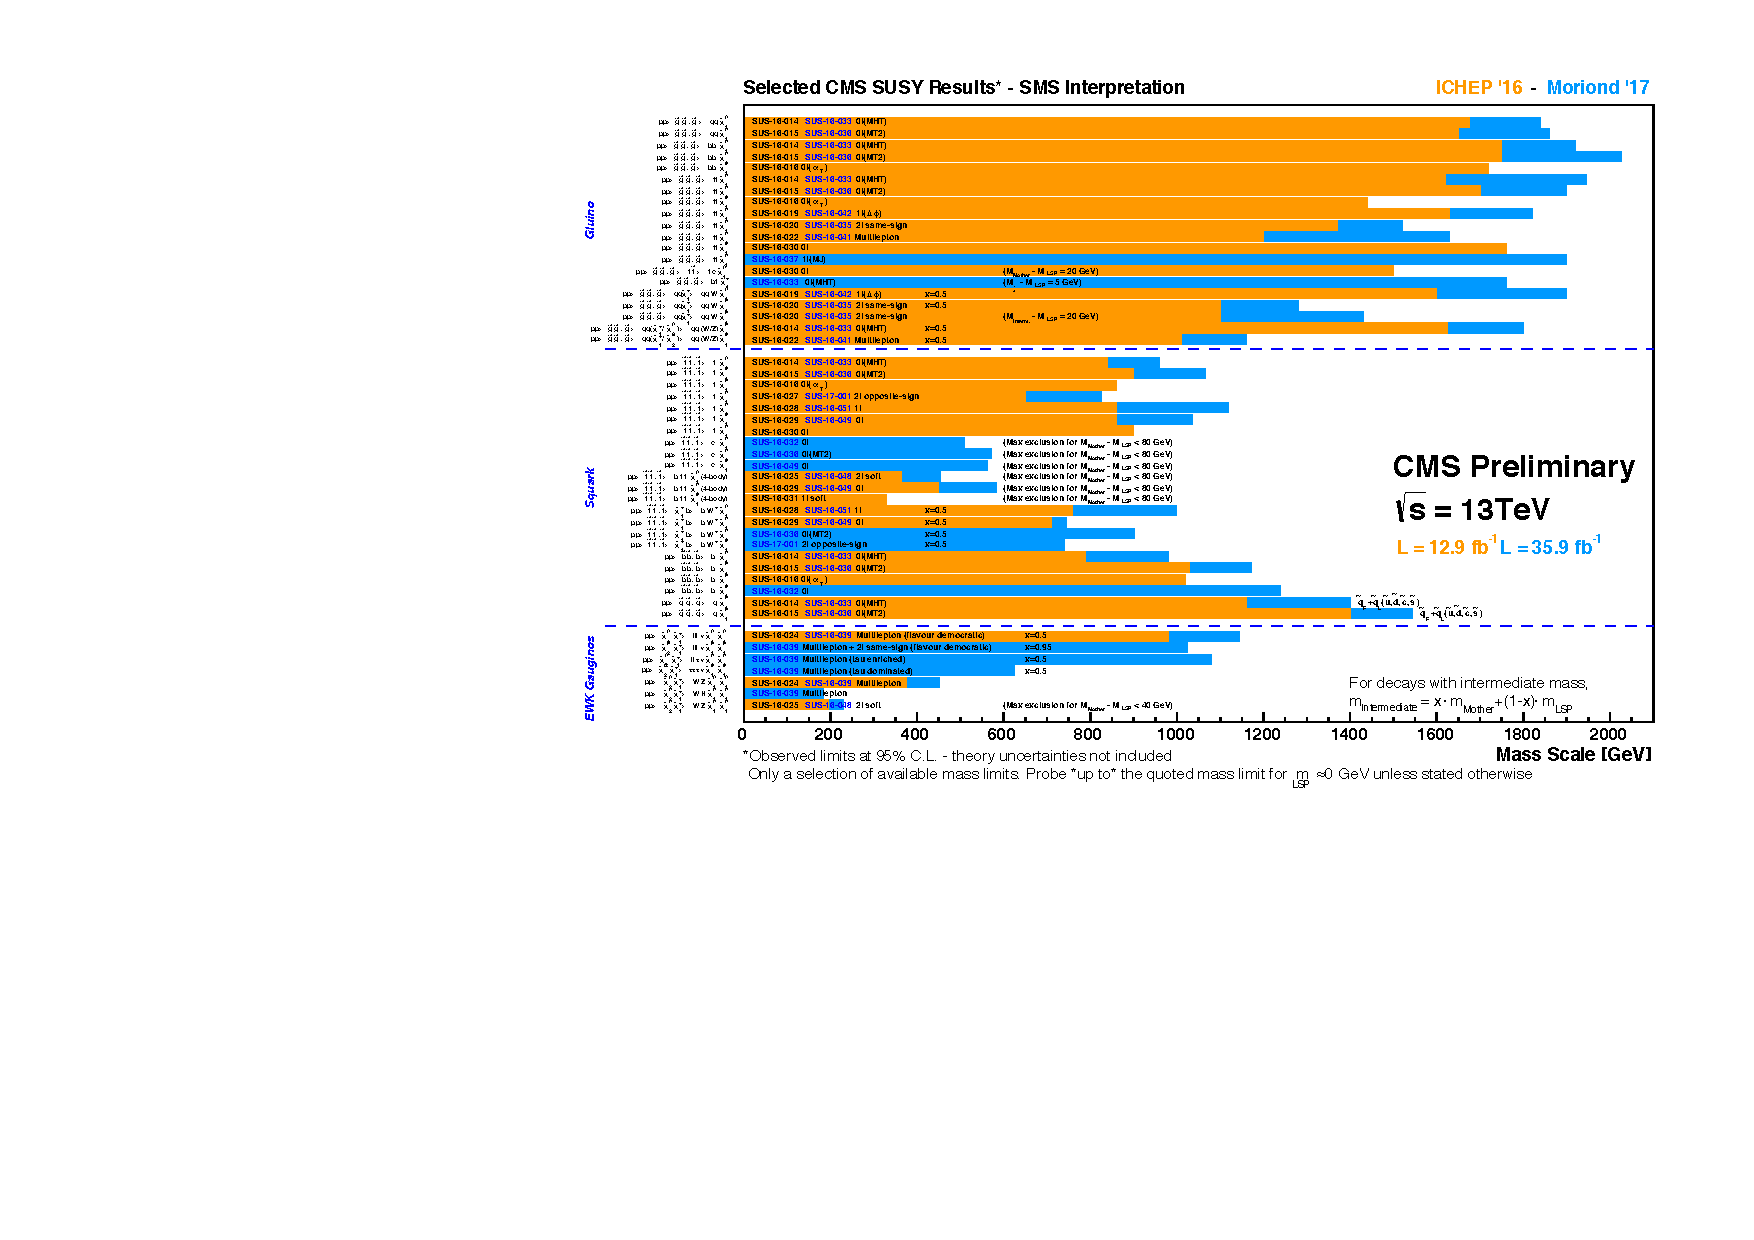
\includegraphics[width=0.93\textwidth]{Plots/SUSY/CMS_Moriond2017_BarPlot}
  \caption{ Best exclusion limits on sparticle masses from searches for SUSY using SMS by ATLAS (top) and CMS (bottom) collaborations \cite{atlasSUSYsummary,cmsSUSYsummary}. In the upper plot, the green bars represent the 7-8 TeV results while the blue bars are summarizing the 13 TeV results. In the lower plot, results summarizing the 13 TeV results, the orange bars represent the~12.9~fb$^{-1}$ results while the blue bars show the~15.9~fb$^{-1}$ results.
  }
  \label{fig:susy_Summary}
\end{figure*}

\begin{figure*}[!hb]
\centering
  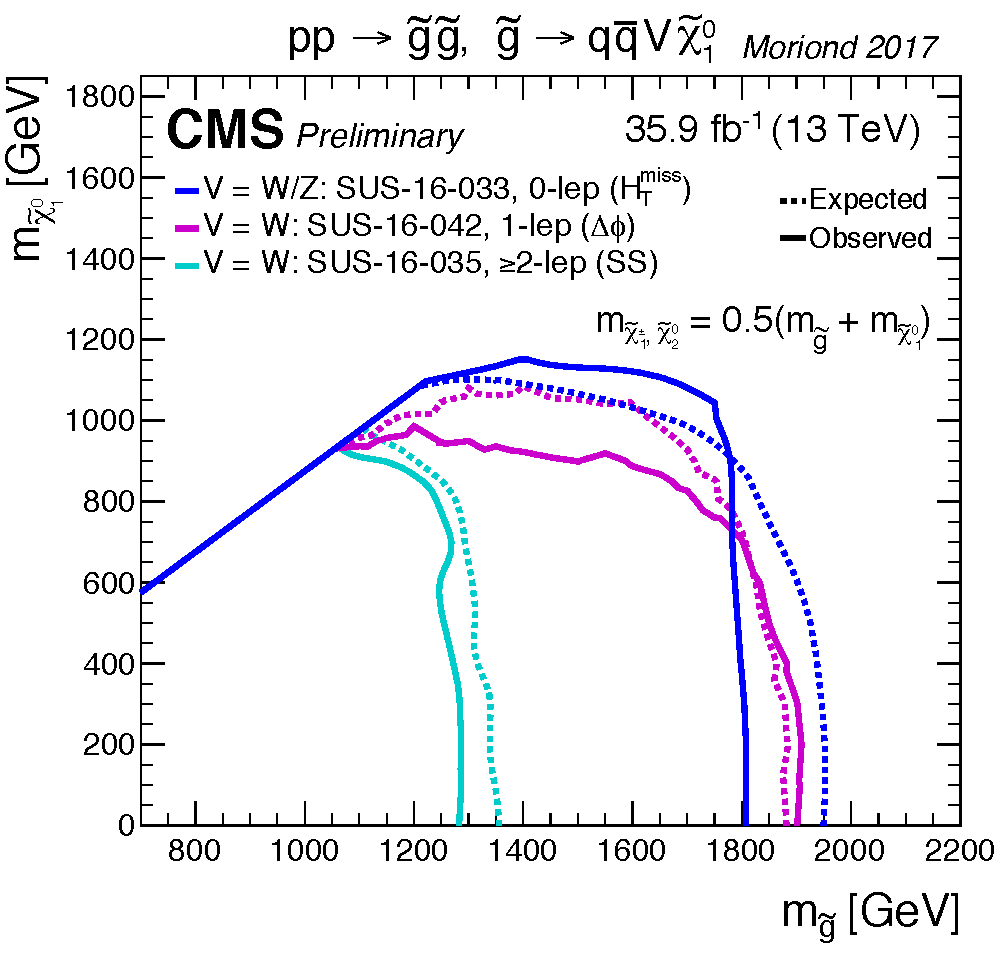
\includegraphics[width=0.45\textwidth]{Plots/SUSY/CMS_SUSY_Strong_1Step}
   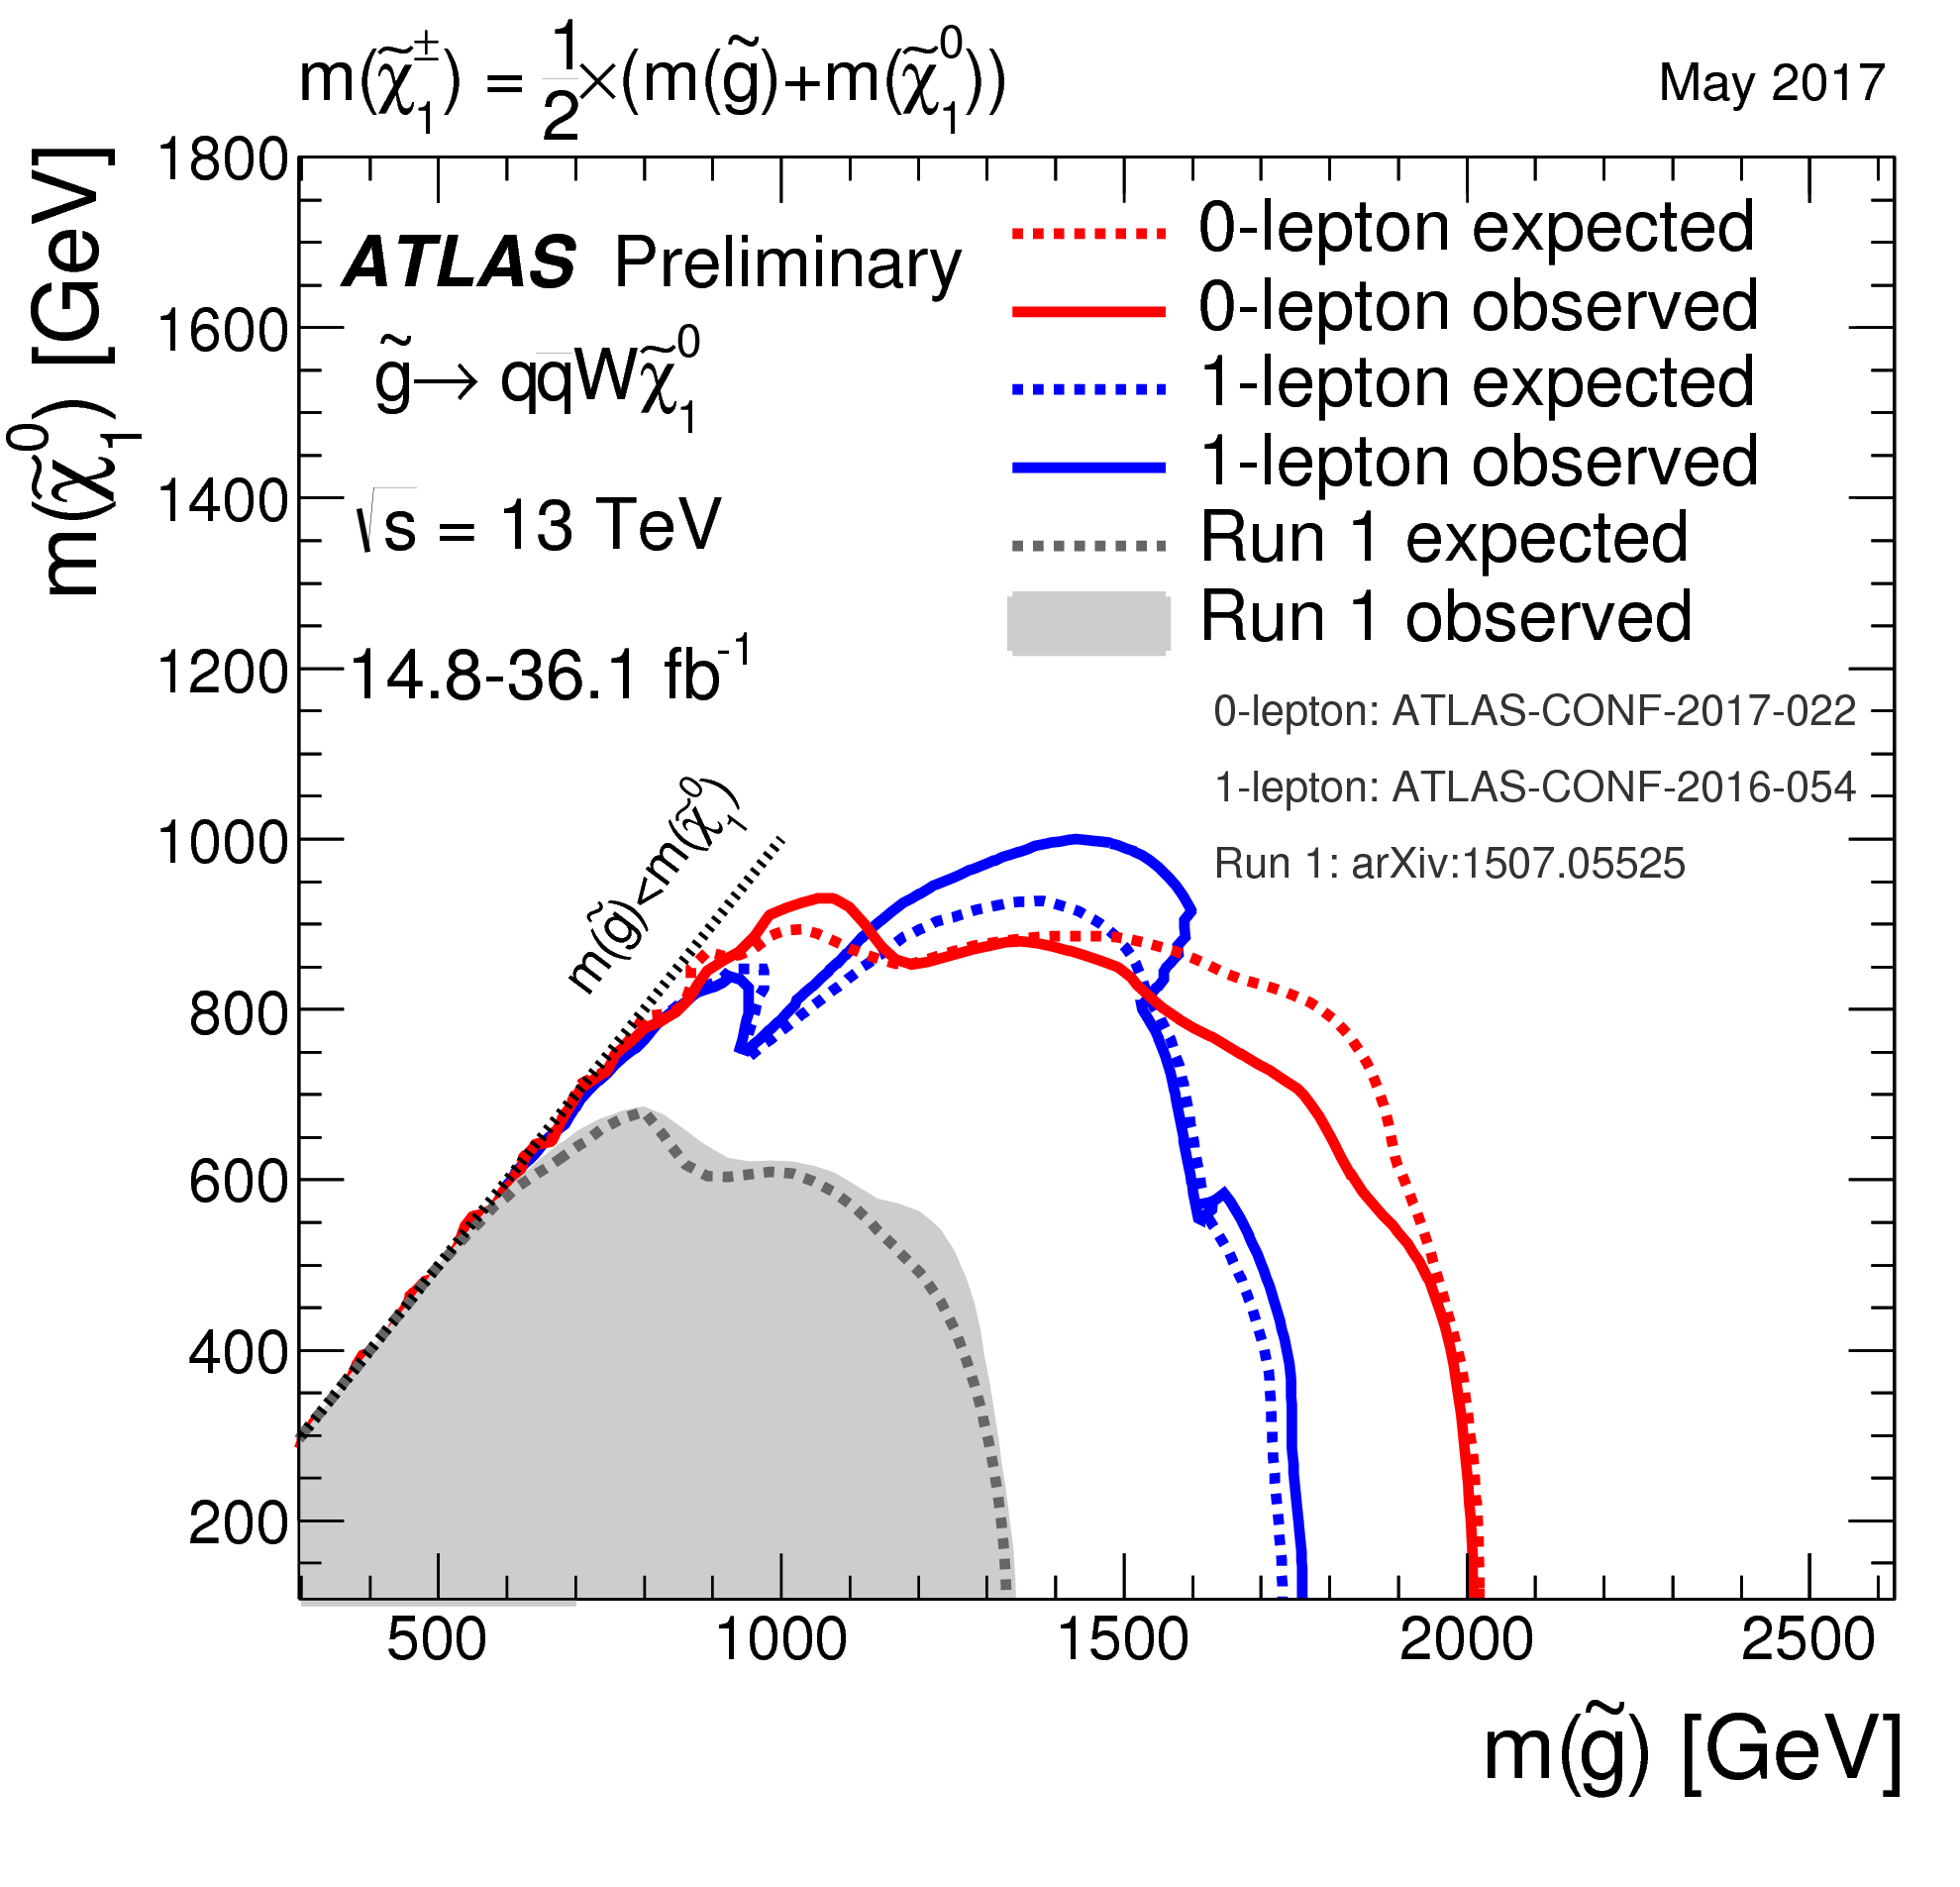
\includegraphics[width=0.45\textwidth]{Plots/SUSY/ATLAS_SUSY_Strong_1step}
  \caption{ 95\% CL exclusion limit curves on the simplified SUSY model of gluino pair production with subsequent decay of $\tilde{g}\rightarrow q\bar{q}WW\ninozero$ obtained by the CMS~(left) and ATLAS~(right) collaborations. The present analysis is corresponding to the result labeled with SUS-16-042.
  }
  \label{fig:SUSY_strong_1step}
\end{figure*}
